%!TEX encoding = UTF-8 Unicode
%!TEX program = xelatex

\documentclass[bachelor]{ustcthesis}
% bachelor|master|doctor
\usepackage{ustcextra}
\graphicspath{{figures/}}
\bibliographystyle{ustcauthoryear}
% \bibliographystyle{ustcnumerical}


\newcommand{\docname}{应用商店系统}
\renewpagestyle{front}[\zihao{-5}]{
    \sethead{}{\docname 需求规格说明书}{}
    \setfoot{}{\thepage}{}
    \headrule
}
\renewpagestyle{main}[\zihao{-5}]{
    \sethead{}{\docname 需求规格说明书}{}
    \setfoot{}{\thepage}{}
    \headrule
}
\newcommand{\HRule}{\rule{\linewidth}{0.5mm}}

\begin{document}




\begin{titlepage}
\begin{center}
~\\[5cm]
\HRule \\[0.4cm]
{\huge \bfseries \docname\\需求规格说明书}\\[0.4cm]
\HRule \\[1.5cm]

\begin{tabular}{ccc}
  & 人员 & 日期 \\ 
  & 董恒 & 2019-4-12 \\
  & 李楠 & 2019-4-12 \\
%拟制 & 张三\ 李四\ 王五 & yyyy-mm-dd \\ 
%评审人 & • & yyyy-mm-dd \\ 
%批准 & • & yyyy-mm-dd \\ 
%签发 & • & yyyy-mm-dd \\ 
\end{tabular} 

\end{center}
\end{titlepage}



\frontmatter
\begin{abstract}
    本说明是软件工程-应用商店系统案例研究项目软件产品的总体设计和实现说明,记
    录了系统整体实现上技术层面上的考虑,并且以需求说明作为依据,同时该文档将作为产品
    实现、特性要求和控制的依据。


    本阶段已在系统的需求分析研究的基础上,对应用商店系统做概要设计。该阶段正式进
入了实际开发阶段,它的目的就是进一步细化软件设计阶段得出的软件总体概貌,把它加工成
在程序细节上非常接近于源程序的软件表示。概要设计说明书主要解决了实现本系统需求的程
序模块设计问题。
\keywords{软件工程\zhspace{}应用商店系统 \zhspace{} 概要设计}

\begin{table}[htbp]
\centering
\caption{缩略词清单} \label{tab:abbr}
\begin{tabular}{|c|c|c|}
    \hline
    缩略语 & 英文全名 & 中文解释 \\
    \hline
    app & application & 应用\\
    \hline
    dev & developer & 开发者 \\
    \hline
    inter & interface & 接口 \\
    \hline
    info & information & 信息 \\
    \hline
    passwd & password & 密码 \\
    \hline
\end{tabular}
\end{table}
    

\end{abstract}

\tableofcontents
\listoffigures
\listoftables
% \listofalgorithms  % 算法索引,如不需要,可直接注释掉本行
% \begin{notation}

%\centering
%XX 软件需求规格说明书

%关键词:能够体现文档描述内容主要方面的词汇。
 
%摘要:


\centering
\begin{tabular}{rl}
$\ln x$ & natural logarithm $\log_ex$ \\
$\log x$ & common logarithm $\log_{10}x$ \\
$x\ \mathrm{mod}\ y$ & remainder \\
\end{tabular}

\end{notation}


\mainmatter
\section{工具简介}
\label{sec:intro}
``违反编码规范的缺陷检测工具''(以下简称本工具)是根据NASAC2018软件原型命题竞赛组 
2018年10月21日晚发布的竞赛题目,
由中国科学技术大学计算机科学与技术学院张昱老师于10月22日
联络2018级硕士研究生张宇翔组队研制。
本参赛队由队长张宇翔、2016级本科生邓胜亮(10月23日加入)、
2018级硕士研究生李森(10月26日加入)组成,
工具研发的起止时间为2018年10月22日至11月10日;
张昱老师进行全程指导。

本参赛队利用 \href{https://clang.llvm.org/}{Clang 7.0.0} 
提供的工具框架
设计实现了具有可配置、易扩展的自动化违反编码规范的缺陷检测工具。
该工具提供函数参数合法性检查、函数错误返回码处理检查、
变量按需初始化检查、头文件自包含检查、循环依赖检查、
函数头注释检查、标识符命名检查等,
产生的诊断信息内容全面、可读性强。
用户可以方便地配置工具的行为,扩展其功能。

\subsection{功能简介}
\label{sec:intro:func}
该工具能够进行的检查如下:

\begin{itemize}
\item {\bf 函数参数合法性检查}
检查代码中模块对外接口是否进行了合法性检查。

\item{\bf 函数错误返回码处理检查}
检查在调用提供了错误指示机制的函数后,是否立即检查了错误指示。

\item{\bf 变量按需初始化检查}
检查代码中是否存在冗余的初始化。

\item{\bf 头文件自包含及循环包含检查}
检查头文件是否自包含且没有循环依赖。

\item{\bf 函数头注释检查}
检查函数头注释风格是否一致、注释中是否只有格式没有内容、是否说明了必要的信息、未注释的函数是否需要补充注释。

\item{\bf 标识符命名检查}
指出函数、变量名中的非英文单词,并对英文变量名提供常见的缩写建议。
\end{itemize}

所有检查的结果在汇报时都会指出其在源码中对应的位置(包括文件路径、行号、列号),方便用户进行修改。
各功能具体的实现细节将在 \S\ref{sec:core} 进行介绍。

\subsection{使用说明简介}
\label{sec:intro:usage}

该工具为命令行工具,用户通过提供命令行参数,对工具进行以下配置:

\begin{itemize}
    \item 关闭指定的一个或多个检查;
    \item 指定英文词典、缩写词典的位置;
    \item 指定返回错误码的函数列表的位置;
    \item 指定要检查的项目的编译命令列表位置;
    \item 指定要检查的文件或目录;
\end{itemize}

除了提供命令行选项以外,用户可以自行删减、扩充英文词典、缩写词典、返回错误码的函数列表,
从而方便地根据实际需要来定制工具的行为。

关于以上配置方式的具体说明见 \S\ref{sec:usage} 一节。

\chapter{总体概述}

本节描述影响产品和产品需求的一般因素。由以下4个部分构成。 有一点需说明的是本节不描述具体的需求,只是使那些将要描述的具体需求更易于理解。
\section{软件概述}
\subsection{项目介绍}
应用商店的开发与时俱进,现在出现的PC端与手机端应用商店出现了严重的割裂,
而且应用的质量得不到保证、用户的反馈得不到及时的回应、开发者的合理权益得不到保障、
用户需要专门花时间去找应用等等问题层出不穷。

现在出现的应用商店无法解决这样问题,这也是本项目出现的主要原因,
即构建一个面向未来的、可拓展的、友好的应用商店系统。
以达到全面替代当前的各种应用商店的目的。


\subsection{产品环境介绍}

本项目构成一个独立的体系而且完全自我包含。

\section{软件功能}
为了便于设计和理解,将软件的功能分为三个组块,即开发者端、服务器端、用户端。


下面详细介绍。

\subsection{开发者端}
针对开发者,我们需要设定开发者是普通的应用程序开发人员甚至是非专业的,为了激发开发的参与,
本系统需要简化应用开发的门槛,因而开发者端需要尽可能简化。
\begin{itemize}
\item 应用管理

	\begin{itemize}
	\item 应⽤上传
	\item 应用更新
	\item 应用删除
	\end{itemize}
\item 信息反馈
	\begin{itemize}
	\item
	应⽤信息查询与管理
	\begin{itemize}
		\item 下载量
		\item 评论
		\item 回复
	\end{itemize}
	\item 收⼊查询与管理
	\begin{itemize}
		\item 提现
		\item 转账
	\end{itemize}
	\end{itemize}

\item \color{red}{应用开发}
	\begin{itemize}
		\item \color{red}{代码编辑}
		\item \color{red}{代码编译与运行}
		\item \color{red}{debug功能}
	\end{itemize}
\end{itemize}
	

\subsection{服务器端}
服务器端是一个增加了某些特殊功能的数据库,需要存储开发者、应用、用户的信息,以及相关的触发操作,
下面的列表详细地说明了其功能。

\begin{itemize}
\item 开发者管理系统
	\begin{itemize}
	\item 开发者信息维护
		\begin{itemize}
		\item 注册与注销
		\item 个人基本信息
		\item 开发的应用
		\end{itemize}
	\item 反馈内容
		\begin{itemize}
			\item 收入查询
			\item 收入提现
			\item 应用评分与评论
		\end{itemize}
	\end{itemize}
\item 应用管理系统
	\begin{itemize}
	\item 应用信息管理
		\begin{itemize}
		\item 基本信息
		\item 下载量
		\item 评价
		\item 评分
		\end{itemize}
	\item 应用上传、更新、删除、下载管理
		\begin{itemize}
			\item 应⽤审核
			\item 应⽤排名
			\item 应⽤推荐
		\end{itemize}
	\end{itemize}
\item ⽤户管理系统
	\begin{itemize}
	\item 用户信息维护
	\begin{itemize}
		\item 注册与注销
		\item 个人基本信息
		\item 下载/购买的应用
	\end{itemize}
	\end{itemize}
\item 第三方管理系统
	\begin{itemize}
	\item ⼴告投放管理
	\item 第三方资助管理
	\item 第三方监督管理
	\end{itemize}
\item \color{red}{应用开发管理系统}
\color{red}{
	\begin{itemize}
		\item 在线开发
		\item 在线预览
	\end{itemize}
}
\end{itemize}
	
\subsection{客户端}
\begin{itemize}
\item 应用管理
	\begin{itemize}
	\item 应⽤查询
	\item 应⽤购买
	\item 应⽤安装
	\item 应⽤更新
	\item 应用删除
	\end{itemize}
\item 信息反馈
	\begin{itemize}
	\item 应用评价
	\begin{itemize}
		\item 评分
		\item 评论
	\end{itemize}
	\end{itemize}
	\color{red}{
		\item 应用个性化
		\begin{itemize}
			\item 个性化配置
			\item 预览
		\end{itemize}	
		}
\end{itemize}

\subsection{需求关系}

\begin{figure}[ht]
	\centering
	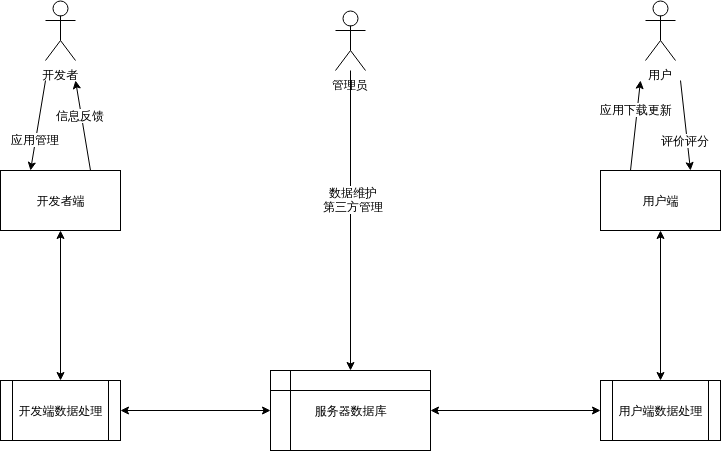
\includegraphics[width=10cm]{top_diagram.png}
	\caption{高层数据流图} \label{fig:top_diagram}
\end{figure}

下面的高层数据流图\ref{fig:top_diagram}简明扼要地说明了三个不同端之间的关系。


\section{用户特征}
开发者应该具有基本的开发能力,任何语言均可,本系统提供不同语言体系的打包与封装。

系统管理员应该具有基本的数据库维护能力。第三方的监督与广告投放应该交由管理员处理。

用户不假设具有任何的专业背景,要求是任何人均可以作为用户来使用本软件系统。


\section{假设和依赖关系}
本项目仅做最基本的假设,依赖于浏览器、网络协议、数据库以及具体的终端设备操作系统。

本项目尽可能面向未来,因而主要使用浏览器作为终端用户的交互设备,所以浏览器协议以及网络协议的改变
会对本项目造成影响。同时,鉴于部分用户的习惯依赖性,也需要提供相应的应用终端。
这一点需要考虑到不同PC或者手机的操作系统的架构。



\chapter{具体需求}
下面详细描述具体的需求。

\section{功能需求}

%本子章节应描述软件产品的输入怎样被转换成输出。它描述了软件必须执行的基本动作。 

%对每一类功能或有时对每一个单独的功能,必须描述输入、处理、输出方面的需求。这些通常以下面四个子段落来组织:
\subsection{开发者端.应用管理}
需求编码为SRS\_Dev\_App\_P01

\subsubsection{介绍}
本小节主要介绍了开发者进行应用管理的需求,包括应用的上传、更新、删除等等。

需求编码为SRS\_Dev\_App\_P01\_F01

\subsubsection{输入}

需求编码为SRS\_Dev\_App\_P01\_I01

针对开发者对其应用的管理需求,其输入数据应当是某个应用和对该应用的操作,数据来源均为开发者,具体如下:

\begin{longtable}[]{@{}ll@{}}
\toprule
数据名称 & 数据要求\tabularnewline
\midrule
\endhead
对应用的操作 & 上传、更新、删除之一\tabularnewline
应用id & 应用id为该开发者开发的应用之一(更新、删除),应用id首次出现(应用上传)\tabularnewline
应用 & 合法的应用程序 \tabularnewline
\bottomrule
\end{longtable}

\subsubsection{处理}
对输入进行处理,得到输出内容,需求编码为SRS\_Dev\_App\_P01\_H01

\textbf{A. 输入数据的有效性检测}

\begin{longtable}[]{@{}ll@{}}
\caption{开发者端进行应用管理输入数据的有效性检测}\label{tab:developer_app_management}\\
\toprule
数据名称 & 数据要求\tabularnewline
\midrule
\endhead
对应用的操作 & 上传、更新、删除之一\tabularnewline
应用id & 应用id为该开发者开发的应用之一(更新、删除),应用id首次出现(应用上传)\tabularnewline
应用 & 合法的应用程序 \tabularnewline
\bottomrule
\end{longtable}

见表\ref{tab:developer_app_management}

\textbf{B. 操作的确切次序,包括各事件的时序}

\begin{figure}[ht]
	\centering
	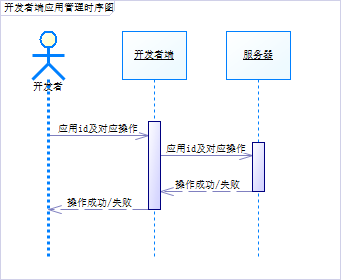
\includegraphics[width=14cm]{developer_app_order.png}
	\caption{开发者端进行应用管理的事件时序} \label{fig:developer_app_order}
\end{figure}
见图\ref{fig:developer_app_order}

\textbf{C. 对异常情况的回应}

\begin{longtable}{|c|p{6cm}|p{6cm}|}
\caption{开发者管理系统异常处理}\label{tab:developer_app_management_exception}\\
\hline
\textbf{异常类型} & \textbf{异常描述} & \textbf{异常处理}\\
\hline
\endfirsthead

\hline
\textbf{异常类型} & \textbf{异常描述} & \textbf{异常处理}\\
\hline
\endhead
\hline 
\endfoot
\hline
\endlastfoot
服务器异常 & 
与服务器采用网络通信,限定时间内没有收到应答 &
储存错误状态,提示开发者检查网络连接\\
应用id不合法 
& 删除或更新应用时,id对应的应用并不存在开发者所开发的应用中
& 提示开发者重新操作\\
应用不合法
& 上传的不是合法的应用程序
&提示开发者重新操作\\
\end{longtable}

表\ref{tab:developer_app_management_exception}概要性描述了几个可能出现的错误,以及相关的解决方案。
更加详细的方案见概要设计。

\textbf{D. 用于把系统输入转换到相应输出的任何方法}
只需要将服务器返回的结果返回给开发者即可,不需要额外的数学算法或操作逻辑等等。
		
\textbf{E. 对输出数据的有效性检测}

此处只考虑开发者端返回e给开发者的数据,返回给服务器的数据参见服务器端.应用管理系统。
输出数据为:操作的成功与否以及可能的错误信息,具体如下:
\begin{longtable}{|p{7cm}|p{7cm}|}
\caption{开发者端应用管理输出有效性检测}\label{tab:concrete_dev_sys_output_valid} \\
\hline
\textbf{输出内容} & \textbf{有效性检测} \\
\hline
\endfirsthead
\hline
\textbf{输出内容} & \textbf{有效性检测} \\
\hline
\endhead
\hline 
\endfoot
\hline
\endlastfoot

操作结果 & 布尔量,成功或失败 \\
错误信息 & 操作成功则为空,操作失败则为一个字符串,建议开发者下一步的操作,长度暂定为128byte\\
\end{longtable}


\subsubsection{输出}
需求编码为SRS\_Dev\_App\_P01\_O01

参见上一节E对输出数据的有效性检测。

\subsection{开发者端.信息反馈}
本小节主要描述了开发者获取信息反馈的需求,比如查询应用评价等等。

需求编码为SRS\_Dev\_Info\_P01

\subsubsection{介绍}
逐条列出与本特性相关的功能需求。包括项目如何响应预期的错误输入,非法条件和无效输入。需求应该简明,完整,不含糊,可验证,必要的。 当需要的信息不确定的时候使用“待定”。
需求编码为SRS\_Dev\_Info\_P01\_F01

\subsubsection{输入}

需求编码为SRS\_Dev\_Info\_P01\_I01
针对开发者获取关于其应用的信息的需求,输入数据应当包括:应用id、具体的查询管理需求等等,数据来源均为开发者(此处不考虑隐式的数据来源,即服务器),具体如下:

\begin{longtable}[]{@{}ll@{}}
\toprule
数据名称 & 数据要求\tabularnewline
\midrule
\endhead
应用id & 应用id为该开发者开发的应用之一\tabularnewline
具体需求 & 应用信息查询、评论回复、收入查询、收入提现、收入转账等命令之一\tabularnewline
评论回复 & 当且仅当具体需求是评论回复时不为空,为一个字符串,长度暂定为256字节\tabularnewline
银行账号 & 当且仅当具体需求是收入提现或转账时不为空,为一个合法的银行账号\tabularnewline
\bottomrule
\end{longtable}

\subsubsection{处理}
对输入进行处理,得到输出内容,
需求编码为SRS\_Dev\_Info\_P01\_H01

\textbf{A. 输入数据的有效性检测}

\begin{longtable}[]{@{}ll@{}}
\caption{开发者端信息反馈的输入数据的有效性检测}\label{tab:developer_app_info}\\
\toprule
数据名称 & 数据要求\tabularnewline
\midrule
\endhead
具体需求 & 应用信息查询、评论回复、收入查询、收入提现、收入转账等命令之一\tabularnewline
应用id & 当且仅当具体需求是应用信息查询时不为空,应用id为该开发者开发的应用之一\tabularnewline
评论回复 & 当且仅当具体需求是评论回复时不为空,为一个字符串,长度暂定为256字节\tabularnewline
银行账号 & 当且仅当具体需求是收入提现或转账时不为空,为一个合法的银行账号\tabularnewline
\bottomrule
\end{longtable}

见表\ref{tab:developer_app_info}

\textbf{B. 操作的确切次序,包括各事件的时序}

\begin{figure}[ht]
	\centering
	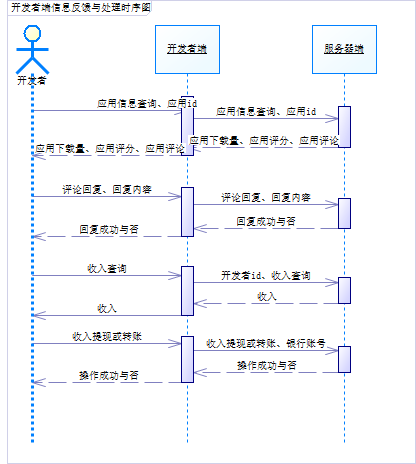
\includegraphics[width=14cm]{developer_info_order.png}
	\caption{开发者获取信息反馈并处理的事件时序} \label{fig:developer_info_order}
\end{figure}
见图\ref{fig:developer_info_order}

\textbf{C. 对异常情况的回应}

\begin{longtable}{|c|p{6cm}|p{6cm}|}
\caption{开发者端信息反馈异常处理}\label{tab:developer_info_exception}\\
\hline
\textbf{异常类型} & \textbf{异常描述} & \textbf{异常处理}\\
\hline
\endfirsthead

\hline
\textbf{异常类型} & \textbf{异常描述} & \textbf{异常处理}\\
\hline
\endhead
\hline 
\endfoot
\hline
\endlastfoot
服务器异常 & 
与服务器采用网络通信,限定时间内没有收到应答 &
储存错误状态,提示开发者检查网络连接\\
应用id不合法 
& id对应的应用并不存在开发者所开发的应用中
& 提示开发者重新操作\\
银行账号不存在
& 用于提现或转账的银行账号不存在
&提示开发者提供正确的银行账号\\
转账或提现金额过大
& 转账或提现金额超过限额
& 提示开发者减小提现或转账金额
\end{longtable}

表\ref{tab:developer_info_exception}概要性描述了几个可能出现的错误,以及相关的解决方案。
更加详细的方案见概要设计。

\textbf{D. 用于把系统输入转换到相应输出的任何方法}
只需要将服务器返回的结果返回给开发者即可,不需要额外的数学算法或操作逻辑等等。
		
\textbf{E. 对输出数据的有效性检测}

此处只考虑开发者端返回给开发者的数据,返回给服务器的数据参见服务器端.应用管理系统。具体如下:
\begin{longtable}{|p{7cm}|p{7cm}|}
\caption{开发者端信息反馈输出有效性检测}\label{tab:concrete_dev_sys_output_valid} \\
\hline
\textbf{输出内容} & \textbf{有效性检测} \\
\hline
\endfirsthead
\hline
\textbf{输出内容} & \textbf{有效性检测} \\
\hline
\endhead
\hline 
\endfoot
\hline
\endlastfoot

下载量 & 整型数据,非负整数 \\
评论 & 字符串\\
收入 & 浮点型数据,非负数\\
操作结果 & 布尔量

\end{longtable}


\subsubsection{输出}
需求编码为SRS\_Dev\_Info\_P01\_O01

参见上一节E对输出数据的有效性检测。


{\color{red}
\subsection{开发者端.应用开发界面}

需求编码为SRS\_Dev\_Dev\_P01
\subsubsection{介绍}
此处提供开发的界面,实现开发-上线一体化,整个应用商店实现完整的生态链。 

为了便于开发,以及免去开发者的下载,
本系统也提供基于浏览器的开发系统。只需与服务器交换数据,就可以使用本系统提供的
编译运行环境。

需求编码为SRS\_Dev\_Dev\_P01\_F01
\subsubsection{输入}

本支系统针对开发者端,数据来源都是开发者端的应用。

需求编码为SRS\_Dev\_Dev\_P01\_I01

输入数据要求

\begin{longtable}[]{@{}ll@{}}
\toprule
数据名称 & 数据要求\tabularnewline
\midrule
\endhead
指令 & 开发界面按键\tabularnewline
code & 通过语法检查  \tabularnewline
\bottomrule
\end{longtable}

\subsubsection{处理}

对输入进行处理,得到输出内容

需求编码为SRS\_Dev\_Dev\_P01\_H01

\textbf{A. 输入数据的有效性检测}

\begin{longtable}[]{@{}ll@{}}
\caption{开发界面输入的有效性检测}\label{tab:dev_dev_input_valid}\\
\toprule
数据名称 & 数据要求\tabularnewline
\midrule
\endhead
指令 & 界面的按键或者命令行并通过简单的语法检查\tabularnewline
code & 通过相应编程语言的语法检查  \tabularnewline
\bottomrule
\end{longtable}

见表\ref{tab:dev_dev_input_valid}

\textbf{B. 操作的确切次序,包括各事件的时序}

由于是在线开发,开发者界面会传输到服务器进行数据的处理,所以其处理的时序也就是先进行简单的语法检查,如果出错,
就直接报错,否则传输到服务器高性能计算中心进行编译运行处理。

\textbf{C. 对异常情况的回应}

\begin{longtable}{|c|p{6cm}|p{6cm}|}
\caption{开发界面异常处理}\label{tab:dev_dev_exception} \\
\hline
\textbf{异常类型} & \textbf{异常描述} & \textbf{异常处理}\\
\hline
\endfirsthead
%\multicolumn{3}{c}{\tablename\ \thetable\ -- \textit{Continued from previous page}} \\
\hline
\textbf{异常类型} & \textbf{异常描述} & \textbf{异常处理}\\
\hline
\endhead
\hline 
%\multicolumn{3}{r}{\textit{Continued on next page}} \\
\endfoot
\hline
\endlastfoot
通信失败 & 
与服务器采用网络通信,限定时间内没有收到应答或者没有新的请求 &
储存错误状态,储存编辑到本地,断开连接\\
语法错误 & 对代码或者命令进行本地语法检查的时候发现语法错误 & 
直接显示出错误信息,并暂停数据传输给服务器\\
攻击检测 & 网络安全相关,比如检测到某个账户持续性注册注销 &
停止对该帐号的应答,并且设定恢复时间\\
\end{longtable}

表\ref{tab:dev_dev_exception}概要性描述了几个可能出现的错误,以及相关的解决方案。
更加详细的方案见概要设计。



\textbf{D. 用于把系统输入转换到相应输出的任何方法}

输入转化成输出,需要经过两个阶段,一是进行语法检查,如果检查出错误,就显示错误信息,
否则传输给服务器编译运行,在返回浏览器数据,并显示。

\textbf{E. 对输出数据的有效性检测}

返回数据无需检查,因为从服务器传输过来的数据为字符或者实时界面数据,可以直接在浏览器上显示。

\subsubsection{输出}

需求编码为SRS\_Dev\_Dev\_P01\_O01

输出数据也就是字符型的信息与界面数据

}




\subsection{服务器端.开发者管理系统}
需求编码为SRS\_Server\_Dev\_P01
\subsubsection{介绍}
集中对开发者的活动进行管理。包括注册与注销,个人基本信息维护,开发的应用列表。
需求编码为SRS\_Server\_Dev\_P01\_F01
\subsubsection{输入}

本支系统针对开发者端,数据来源都是开发者端的应用

需求编码为SRS\_Server\_Dev\_P01\_I01

输入数据要求

\begin{longtable}[]{@{}ll@{}}
\toprule
数据名称 & 数据要求\tabularnewline
\midrule
\endhead
用户名 & 可以接收验证码的邮箱\tabularnewline
密码 &
至少8个字符;必须包含大写与小写字母;至少一个数字;\tabularnewline
\bottomrule
\end{longtable}

输入数据根据不同功能需求的开发者端口要求

\begin{longtable}[]{@{}lll@{}}
\toprule
开发者端功能需求 & 用户名 & 密码\tabularnewline
\midrule
\endhead
注册 & YES & NO\tabularnewline
登录 & YES & YES\tabularnewline
注销 & YES & YES\tabularnewline
找回密码 & YES & NO\tabularnewline
\bottomrule
\end{longtable}

\subsubsection{处理}

对输入进行处理,得到输出内容

需求编码为SRS\_Server\_Dev\_P01\_H01

\textbf{A. 输入数据的有效性检测}

\begin{longtable}[]{@{}ll@{}}
\caption{开发者系统输入的有效性检测}\label{tab:developer_sys_input_valid}\\
\toprule
数据名称 & 数据要求\tabularnewline
\midrule
\endhead
用户名 & 含有@的正常邮箱,是否能接收验证码在此处的初始检测不作要求\tabularnewline
密码 &
至少8个字符;必须包含大写与小写字母;至少一个数字;\tabularnewline
\bottomrule
\end{longtable}

见表\ref{tab:developer_sys_input_valid}

\textbf{B. 操作的确切次序,包括各事件的时序}

\begin{figure}[ht]
	\centering
	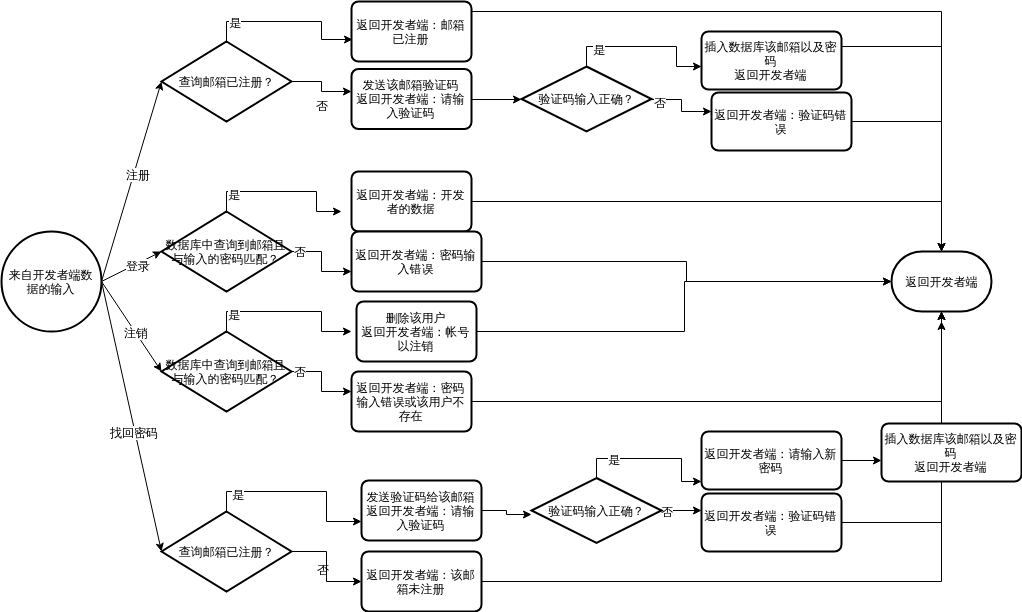
\includegraphics[width=14cm]{concrete_dev_sys.png}
	\caption{开发者管理系统事件时序} \label{fig:concrete_developer}
\end{figure}


数据流图\ref{fig:concrete_developer}明确表示了开发者管理系统的运行


\textbf{C. 对异常情况的回应}

\begin{longtable}{|c|p{6cm}|p{6cm}|}
\caption{开发者管理系统异常处理}\label{tab:developer_exception} \\
\hline
\textbf{异常类型} & \textbf{异常描述} & \textbf{异常处理}\\
\hline
\endfirsthead
%\multicolumn{3}{c}{\tablename\ \thetable\ -- \textit{Continued from previous page}} \\
\hline
\textbf{异常类型} & \textbf{异常描述} & \textbf{异常处理}\\
\hline
\endhead
\hline 
%\multicolumn{3}{r}{\textit{Continued on next page}} \\
\endfoot
\hline
\endlastfoot
通信失败 & 
与开发者端采用网络通信,限定时间内没有收到应答或者没有新的请求 &
储存错误状态,断开连接\\
数据库异常 & 数据库出现异常,比如数据库断联,数据库储存满 &
暂停服务,通知管理员\\
攻击检测 & 网络安全相关,比如检测到某个账户持续性注册注销 &
停止对该帐号的应答,并且设定恢复时间\\
\end{longtable}

表\ref{tab:developer_exception}概要性描述了几个可能出现的错误,以及相关的解决方案。
更加详细的方案见概要设计。



\textbf{D. 用于把系统输入转换到相应输出的任何方法}

开发者系统的处理主要是对数据库的访问处理,根据数据流图\ref{fig:concrete_developer}的
业务逻辑处理即可,并不需要额外的方程式或者数学算法。
		
\textbf{E. 对输出数据的有效性检测}

输出内容分为两类,一是返回给开发者端的提示与错误信息:主体为文本内容,并且为每个信息配有unsigned int类型的描述符。
相关信息有:邮箱已注册;邮箱未注册;输入验证码;密码错误;

\begin{longtable}{|p{7cm}|p{7cm}|}
\caption{开发者管理系统输出有效性检测}\label{tab:concrete_dev_sys_output_valid} \\
\hline
\textbf{输出内容} & \textbf{有效性检测} \\
\hline
\endfirsthead
%\multicolumn{2}{c}{\tablename\ \thetable\ -- \textit{Continued from previous page}} \\
\hline
\textbf{输出内容} & \textbf{有效性检测} \\
\hline
\endhead
\hline 
%\multicolumn{2}{r}{\textit{Continued on next page}} \\
\endfoot
\hline
\endlastfoot

用户名 & 不为空,默认为邮箱,可进行修改 \\
姓名 & 不为空,中文或英文字符串,Unicode格式,限制长度64bytes \\
性别 & 可为空,男/女 \\
年龄 & 可为空,类型为unsigned int \\
开发的应用ID & 可为空,类型为unsigned int, 全局唯一code \\
收入查询 & 不可为空,类型为unsigned int, 如果没有收益则为0 \\
收入提现 & 可为空,提现码,需要与银行账户、支付宝、微信等接入 \\
应用评分与评价 & 可为空,返回一个表格,主码为应用ID, 评分为0~5区间的float类型,评价为字符串序列 \\

\end{longtable}


另外就是返回开发者的信息,
见表\ref{tab:concrete_dev_sys_output_valid}

\subsubsection{输出}

需求编码为SRS\_Server\_Dev\_P01\_O01

\begin{longtable}{|p{3cm}|p{4cm}|p{1cm}|p{6cm}|}
\caption{开发者管理系统输出}\label{tab:concrete_dev_sys_output} \\
\hline
\textbf{输出内容} & \textbf{输出位置} & \textbf{数量}  & \textbf{非法值处理错误信息}    \\
\hline
\endfirsthead
%\multicolumn{4}{c}{\tablename\ \thetable\ -- \textit{Continued from previous page}} \\
\hline
\textbf{输出内容} & \textbf{输出位置} & \textbf{数量}  & \textbf{非法值处理错误信息}  \\
\hline
\endhead
\hline 
%\multicolumn{4}{r}{\textit{Continued on next page}} \\
\endfoot
\hline
\endlastfoot

用户名 & 开发者端 & 1 & 用户名不存在\\
姓名 & 开发者端 & 1 & 姓名字符含有非法字符\\
性别 & 开发者端 & 0/1 & 无\\
年龄 & 开发者端 & 0/1 & 无\\
开发的应用ID & 开发者端 & $\ge 0$ & 无\\
收入查询 & 开发者端 & 1 & 无\\
收入提现 & 开发者端 & 0/1 & 无\\
应用评分与评价 & 开发者端 & $\ge 0$ & 无\\
注册的用户名密码 & 数据库 & 1 & 该用户已注册\\
注销的用户名密码 & 数据库 & 1 & 该用户未注册 \\

\end{longtable}
	
对输出数据的管理见表\ref{tab:concrete_dev_sys_output}




\subsection{服务器端.应用管理系统}
需求编码为SRS\_Server\_App\_P01

\subsubsection{介绍}
集中对应用数据的的管理,包括两大方面,一是应用信息的维护与更新,二是应用本身的上传、更新、下载、删除管理。

需求编码为SRS\_Server\_App\_P01\_F01

\subsubsection{输入}

需求编码为SRS\_Server\_App\_P01\_I01

\begin{longtable}{|p{3cm}|p{4cm}|p{1cm}|p{6cm}|}
\caption{应用管理系统输入}\label{tab:concrete_app_sys_input} \\
\hline
\textbf{输入内容} & \textbf{输入来源} & \textbf{数量}  & \textbf{有效范围}    \\
\hline
\endfirsthead
%\multicolumn{4}{c}{\tablename\ \thetable\ -- \textit{Continued from previous page}} \\
\hline
\textbf{输入内容} & \textbf{输入来源} & \textbf{数量}  & \textbf{有效范围}  \\
\hline
\endhead
\hline 
%\multicolumn{4}{r}{\textit{Continued on next page}} \\
\endfoot
\hline
\endlastfoot

开发者登录并提取应用信息 & 开发者端 & 1 & 系统内部定义开发者登录成功的描述符 \\
开发者登录并上传应用 & 开发者端 & 1 & 应用的合法性 \\
开发者登录并更新应用 & 开发者端 & 1 & 应用的合法性 \\
开发者登录并删除应用 & 开发者端 & 1 & 应用属于该开发者 \\
用户登录并搜索应用名 & 用户端 & 1 & 系统内部定义用户登录成功的描述符 \\
用户登录并查看购买的应用 & 用户端 & 1 & 系统内部定义用户登录成功的描述符 \\
游客搜索应用名 & 用户端 & 1 & 任何字符 \\
游客查看应用的下载量/评分/评价 & 用户端 &1 & 该应用存在 \\

\end{longtable}


对输入的管理信息见表\ref{tab:concrete_app_sys_input}	

\subsubsection{处理}
包含对输入数据所执行的所有操作和如何获得输出的过程

需求编码为SRS\_Server\_App\_P01\_H01

\textbf{A. 输入数据的有效性检测}

\begin{longtable}{|p{3cm}|p{11cm}|}
\caption{应用管理系统输入有效性检测}\label{tab:concrete_app_sys_input_valid} \\
\hline
\textbf{输入内容} & \textbf{有效性检测}    \\
\hline
\endfirsthead
%\multicolumn{2}{c}{\tablename\ \thetable\ -- \textit{Continued from previous page}} \\
\hline
\textbf{输入内容} & \textbf{有效性检测}   \\
\hline
\endhead
\hline 
%\multicolumn{2}{r}{\textit{Continued on next page}} \\
\endfoot
\hline
\endlastfoot
开发者登录 & 符合登录描述符规范 \\
用户登录 & 符合登录描述符规范 \\
应用名搜索 & 任何字符 \\
应用上载 & 符合应用程序规范的应用,后期需要接受应用审查 \\
评分 & 0-5 unsigned int \\
评价 & 字符串,unicode,128 bytes \\
\end{longtable}
	
输入数据的有效性检测见表\ref{tab:concrete_app_sys_input_valid}


\textbf{B. 操作的确切次序,包括各事件的时序}

\begin{figure}[ht]
	\centering
	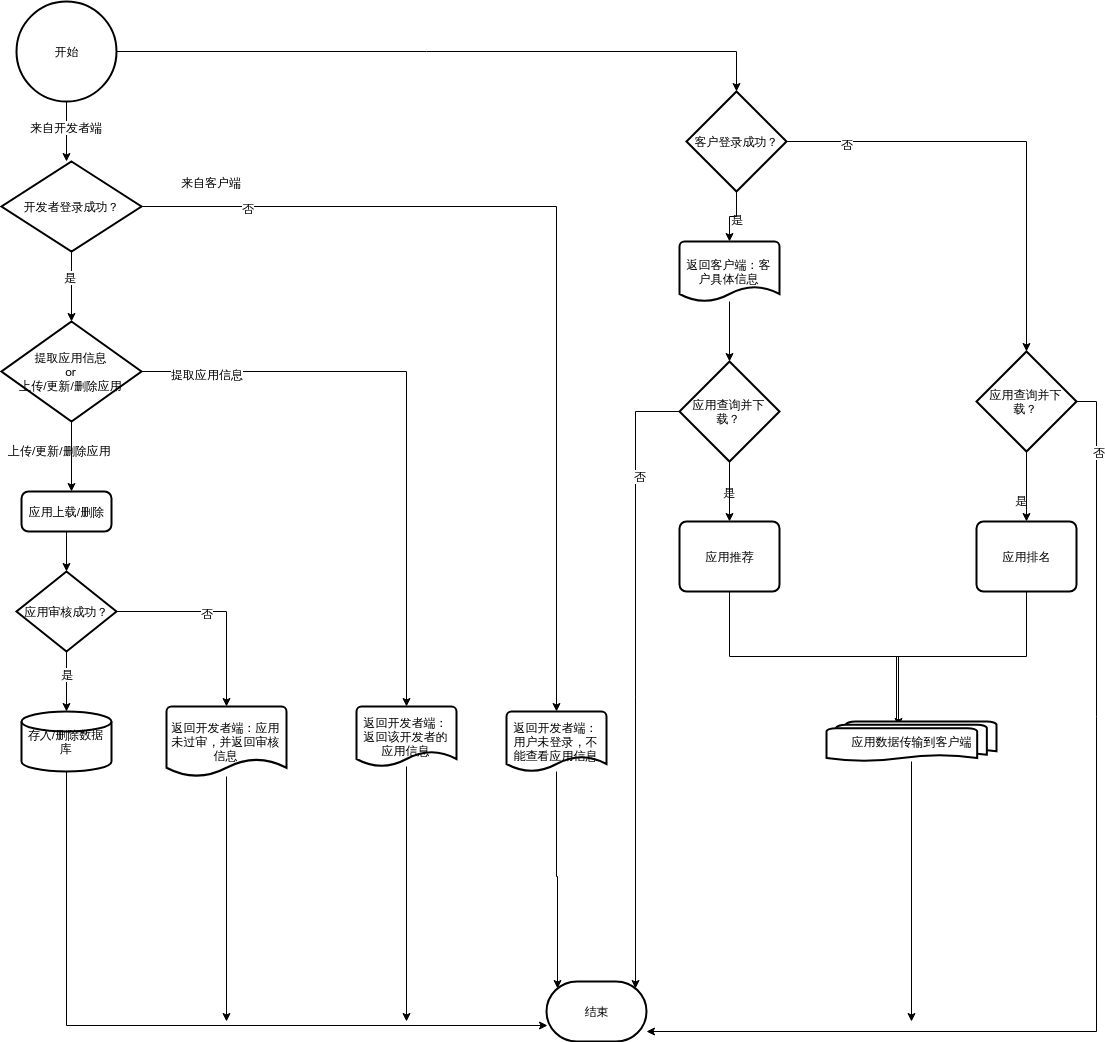
\includegraphics[width=14cm]{concrete_app_sys.png}
	\caption{应用管理系统事件时序} \label{fig:concrete_app_sys}
\end{figure}

对应用管理系统的事件时序见图\ref{fig:concrete_app_sys}

\textbf{C. 对异常情况的回应}

\begin{longtable}{|p{3cm}|p{5cm}|p{6cm}|}
\caption{应用管理系统异常处理}\label{tab:concrete_app_sys_exception} \\
\hline
\textbf{异常类型} & \textbf{异常描述} & \textbf{异常处理}\\
\hline
\endfirsthead
%\multicolumn{3}{c}{\tablename\ \thetable\ -- \textit{Continued from previous page}} \\
\hline
\textbf{异常类型} & \textbf{异常描述} & \textbf{异常处理}\\
\hline
\endhead
\hline 
%\multicolumn{3}{r}{\textit{Continued on next page}} \\
\endfoot
\hline
\endlastfoot
通信失败 & 
与开发者或用户端端采用网络通信,限定时间内没有收到应答或者没有新的请求 &
储存错误状态,断开连接\\
数据库异常 & 数据库出现异常,比如数据库断联,数据库储存满 &
暂停服务,通知管理员\\
攻击检测 & 网络安全相关,比如检测到某个账户持续性刷评 &
停止对该帐号的应答,并且设定恢复时间\\
\end{longtable}

表\ref{tab:concrete_app_sys_exception}概要性描述了几个可能出现的错误,以及相关的解决方案。
更加详细的方案见概要设计。


\textbf{D. 用于把系统输入转换到相应输出的任何方法}

\begin{longtable}{|p{3cm}|p{11cm}|}
\caption{应用管理系统转换处理}\label{tab:concrete_app_sys_transform} \\
\hline
\textbf{过程名} & \textbf{处理方式} \\
\hline
\endfirsthead
%\multicolumn{2}{r}{\tablename\ \thetable\ -- \textit{Continued from previous page}} \\
\hline
\textbf{过程名} & \textbf{处理方式}\\
\hline
\endhead
\hline 
%\multicolumn{2}{r}{\textit{Continued on next page}} \\
\endfoot
\hline
\endlastfoot
应用审核 & 采用AI审核与人工审核结合的办法。 AI审核包括试运行、关键词检测、内容分析、抄袭检测、评分估计等方式;
人工审核指AI审核后不通过返回给开发者,并且开发者提出异议的时候人工检测\\
应用排名 & 针对未登录的游客,主体按照用户评分推荐,给新出的应用分流,给持续增加使用人数与评分的应用更多流量 \\
应用推荐 & 针对已经登录的用户,除了使用应用排名给出的应用推荐,还要结合用户的使用习惯以及同龄人的喜好给予推荐 \\

\end{longtable}
		
\textbf{E.	对输出数据的有效性检测}

\begin{longtable}{|p{3cm}|p{11cm}|}
\caption{应用管理系统输出有效性检测}\label{tab:concrete_app_sys_output_valid} \\
\hline
\textbf{输出内容} & \textbf{有效性检测}    \\
\hline
\endfirsthead
%\multicolumn{2}{c}{\tablename\ \thetable\ -- \textit{Continued from previous page}} \\
\hline
\textbf{输出内容} & \textbf{有效性检测}   \\
\hline
\endhead
\hline 
%\multicolumn{2}{r}{\textit{Continued on next page}} \\
\endfoot
\hline
\endlastfoot
应用下载数据 & MD5检验未损坏 \\
搜索获得的应用列表 & 包含应用名、应用ID、应用图片、应用简介、应用评分与评价\\
开发者的应用列表 & 除了上述内容外,还包含应用的更新记录、下载量分析、评分分析、评价分类汇总\\
\end{longtable}
对输出的有效性检测见表\ref{tab:concrete_app_sys_output_valid}


\subsubsection{输出}

需求编码为SRS\_Server\_App\_P01\_O01

\begin{longtable}{|p{3cm}|p{4cm}|p{1cm}|p{6cm}|}
\caption{应用管理系统输出}\label{tab:concrete_app_sys_output} \\
\hline
\textbf{输出内容} & \textbf{输出位置} & \textbf{数量}  & \textbf{非法值处理错误信息}    \\
\hline
\endfirsthead
%\multicolumn{4}{c}{\tablename\ \thetable\ -- \textit{Continued from previous page}} \\
\hline
\textbf{输出内容} & \textbf{输出位置} & \textbf{数量}  & \textbf{非法值处理错误信息}  \\
\hline
\endhead
\hline 
%\multicolumn{4}{r}{\textit{Continued on next page}} \\
\endfoot
\hline
\endlastfoot
应用下载数据 & 用户端 & 1 & 重新传输数据\\
搜索获得的应用列表 & 用户端 & $\ge 0$ & 不存在时返回0\\
开发者的应用列表 & 用户端 & $\ge 0$ & 不存在时返回0\\
\end{longtable}
	
对输出数据的管理见表\ref{tab:concrete_app_sys_output}


\subsection{服务器端.用户管理系统}
需求编码为SRS\_Server\_User\_P01
\subsubsection{介绍}
集中对用户的活动进行管理。包括注册与注销,个人基本信息维护,下载/购买的应用列表。

需求编码为SRS\_Server\_App\_P01\_F01
\subsubsection{输入}

需求编码为SRS\_Server\_App\_P01\_I01

本支系统针对用户端,数据来源都是用户端的应用

输入数据要求

\begin{longtable}[]{@{}ll@{}}
\toprule
数据名称 & 数据要求\tabularnewline
\midrule
\endhead
用户名 & 可以接收验证码的邮箱\tabularnewline
密码 &
至少8个字符;必须包含大写与小写字母;至少一个数字;\tabularnewline
\bottomrule
\end{longtable}

输入数据根据不同功能需求的用户端口要求

\begin{longtable}[]{@{}lll@{}}
\toprule
用户端功能需求 & 用户名 & 密码\tabularnewline
\midrule
\endhead
注册 & YES & NO\tabularnewline
登录 & YES & YES\tabularnewline
注销 & YES & YES\tabularnewline
找回密码 & YES & NO\tabularnewline
免费应用下载 & NO & NO \tabularnewline
\bottomrule
\end{longtable}

\subsubsection{处理}

对输入进行处理,得到输出内容

需求编码为SRS\_Server\_App\_P01\_H01

\textbf{A. 输入数据的有效性检测}

\begin{longtable}[]{@{}ll@{}}
\caption{用户系统输入的有效性检测}\label{tab:concrete_user_sys_input_valid}\\
\toprule
数据名称 & 数据要求\tabularnewline
\midrule
\endhead
用户名 & 含有@的正常邮箱,是否能接收验证码在此处的初始检测不作要求\tabularnewline
密码 &
至少8个字符;必须包含大写与小写字母;至少一个数字;\tabularnewline
\bottomrule
\end{longtable}

见表\ref{tab:concrete_user_sys_input_valid}

\textbf{B. 操作的确切次序,包括各事件的时序}

\begin{figure}[ht]
	\centering
	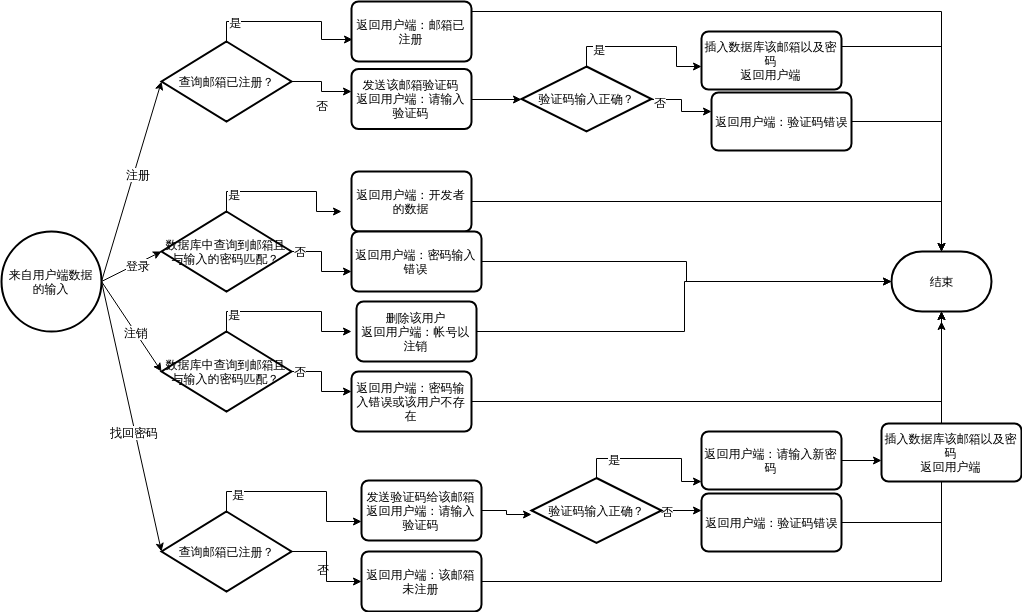
\includegraphics[width=14cm]{concrete_user_sys.png}
	\caption{用户管理系统事件时序} \label{fig:concrete_user_sys}
\end{figure}


数据流图\ref{fig:concrete_user_sys}明确表示了用户管理系统的运行


\textbf{C. 对异常情况的回应}

\begin{longtable}{|c|p{6cm}|p{6cm}|}
\caption{用户管理系统异常处理}\label{tab:developer_exception} \\
\hline
\textbf{异常类型} & \textbf{异常描述} & \textbf{异常处理}\\
\hline
\endfirsthead
%\multicolumn{3}{c}{\tablename\ \thetable\ -- \textit{Continued from previous page}} \\
\hline
\textbf{异常类型} & \textbf{异常描述} & \textbf{异常处理}\\
\hline
\endhead
\hline 
%\multicolumn{3}{r}{\textit{Continued on next page}} \\
\endfoot
\hline
\endlastfoot
通信失败 & 
与用户端采用网络通信,限定时间内没有收到应答或者没有新的请求 &
储存错误状态,断开连接\\
数据库异常 & 数据库出现异常,比如数据库断联,数据库储存满 &
暂停服务,通知管理员\\
攻击检测 & 网络安全相关,比如检测到某个账户持续性注册注销 &
停止对该帐号的应答,并且设定恢复时间\\
\end{longtable}

表\ref{tab:developer_exception}概要性描述了几个可能出现的错误,以及相关的解决方案。
更加详细的方案见概要设计。



\textbf{D. 用于把系统输入转换到相应输出的任何方法}

用户系统的处理主要是对数据库的访问处理,根据数据流图\ref{fig:concrete_user_sys}的
业务逻辑处理即可,并不需要额外的方程式或者数学算法。
		
\textbf{E. 对输出数据的有效性检测}

输出内容分为两类,一是返回给用户端的提示与错误信息:主体为文本内容,并且为每个信息配有unsigned int类型的描述符。
相关信息有:邮箱已注册;邮箱未注册;输入验证码;密码错误;

\begin{longtable}{|p{7cm}|p{7cm}|}
\caption{用户管理系统输出有效性检测}\label{tab:concrete_user_sys_output_valid} \\
\hline
\textbf{输出内容} & \textbf{有效性检测} \\
\hline
\endfirsthead
%\multicolumn{2}{c}{\tablename\ \thetable\ -- \textit{Continued from previous page}} \\
\hline
\textbf{输出内容} & \textbf{有效性检测} \\
\hline
\endhead
\hline 
%\multicolumn{2}{r}{\textit{Continued on next page}} \\
\endfoot
\hline
\endlastfoot
用户名 & 不为空,默认为邮箱,可进行修改 \\
姓名 & 不为空,中文或英文字符串,Unicode格式,限制长度64bytes \\
性别 & 可为空,男/女 \\
年龄 & 可为空,类型为unsigned int \\
下载/购买的应用ID & 可为空,类型为unsigned int, 全局唯一code \\
\end{longtable}


另外就是返回用户的信息,
见表\ref{tab:concrete_user_sys_output_valid}

\subsubsection{输出}

需求编码为SRS\_Server\_App\_P01\_O01

\begin{longtable}{|p{3cm}|p{4cm}|p{1cm}|p{6cm}|}
\caption{用户管理系统输出}\label{tab:concrete_user_sys_output} \\
\hline
\textbf{输出内容} & \textbf{输出位置} & \textbf{数量}  & \textbf{非法值处理错误信息}    \\
\hline
\endfirsthead
%\multicolumn{4}{c}{\tablename\ \thetable\ -- \textit{Continued from previous page}} \\
\hline
\textbf{输出内容} & \textbf{输出位置} & \textbf{数量}  & \textbf{非法值处理错误信息}  \\
\hline
\endhead
\hline 
%\multicolumn{4}{r}{\textit{Continued on next page}} \\
\endfoot
\hline
\endlastfoot
用户名 & 用户端 & 1 & 用户名不存在\\
姓名 & 用户端 & 1 & 姓名字符含有非法字符\\
性别 & 用户端 & 0/1 & 无\\
年龄 & 用户端 & 0/1 & 无\\
下载/购买的应用ID & 用户端 & $\ge 0$ & 无\\
注册的用户名密码 & 数据库 & 1 & 该用户已注册\\
注销的用户名密码 & 数据库 & 1 & 该用户未注册 \\
\end{longtable}
	
对输出数据的管理见表\ref{tab:concrete_user_sys_output}

\subsection{服务器端.第三方管理系统}

需求编码为SRS\_Server\_Other\_P01
\subsubsection{介绍}
第三方用户主要是广告投放、监督、资助,用户权限很大而且用户很少,不应当对外提供接口,
而应当交由管理员处理。

需求编码为SRS\_Server\_Other\_P01\_F01

\subsubsection{输入}

需求编码为SRS\_Server\_Other\_P01\_I01

\begin{longtable}{|p{3cm}|p{4cm}|p{1cm}|p{6cm}|}
\caption{第三方管理系统输入}\label{tab:concrete_other_sys_input} \\
\hline
\textbf{输入内容} & \textbf{输入来源} & \textbf{数量}  & \textbf{有效范围}    \\
\hline
\endfirsthead
%\multicolumn{4}{c}{\tablename\ \thetable\ -- \textit{Continued from previous page}} \\
\hline
\textbf{输入内容} & \textbf{输入来源} & \textbf{数量}  & \textbf{有效范围}  \\
\hline
\endhead
\hline 
%\multicolumn{4}{r}{\textit{Continued on next page}} \\
\endfoot
\hline
\endlastfoot
广告 & 广告投放机构 & $\ge 0$ & 符合法律的广告内容 \\
资助 & 公益单位或个人或广告投放机构 & $\ge 0$ & 符合转账条款 \\
监督 & 官方或公司 & &\\
\end{longtable}
对输入的管理信息见表\ref{tab:concrete_other_sys_input}	

\subsubsection{处理}
包含对输入数据所执行的所有操作和如何获得输出的过程

需求编码为SRS\_Server\_Other\_P01\_H01

\textbf{A. 输入数据的有效性检测}

交由管理员处理,此处不需要

\textbf{B. 操作的确切次序,包括各事件的时序}

交由管理员处理,此处不需要

\textbf{C. 对异常情况的回应}

交由管理员处理,此处不需要

\textbf{D. 用于把系统输入转换到相应输出的任何方法}

		
\textbf{E.	对输出数据的有效性检测}

交由管理员处理,此处不需要

\subsubsection{输出}

需求编码为SRS\_Server\_Other\_P01\_O01

交由管理员处理,此处不需要

{\color{red}

\subsection{服务器端.应用开发管理系统}

需求编码为SRS\_Server\_DevSys\_P01
\subsubsection{介绍}
集中处理开发者端的开发界面和用户端的个性化界面的数据计算,包括编译执行、debug.

处理完的数据需要传输给开发者端或者用户端显示给客户。

需求编码为SRS\_Server\_DevSys\_P01\_F01
\subsubsection{输入}

需求编码为SRS\_Server\_DevSys\_P01\_I01

本支系统针对开发者端和用户端,数据来源都是相应的开发或个性化界面。

输入数据要求

\begin{longtable}[]{@{}ll@{}}
\toprule
数据名称 & 数据要求\tabularnewline
\midrule
\endhead
命令 & 经过语法检查的指令,拥有执行权限,并且可执行\tabularnewline
代码 &
经过语法检查的字符串\tabularnewline
配置 & 由相应应用提供的对外配置接口 \tabularnewline
\bottomrule
\end{longtable}


\subsubsection{处理}

对输入进行处理,得到输出内容

需求编码为SRS\_Server\_DevSys\_P01\_H01

\textbf{A. 输入数据的有效性检测}

\begin{longtable}[]{@{}ll@{}}
\caption{应用开发管理系统输入的有效性检测}\label{tab:concrete_DevSyS_input_valid}\\
\toprule
数据名称 & 数据要求\tabularnewline
\midrule
\endhead
命令 & 拥有执行权限,并且可执行\tabularnewline
代码 & 不含攻击特征 \tabularnewline
配置 & 符合接口特征且不含攻击特征 \tabularnewline
\bottomrule
\end{longtable}

见表\ref{tab:concrete_DevSyS_input_valid}

\textbf{B. 操作的确切次序,包括各事件的时序}

分成两类事件,来自开发者端的应用开发界面或者来自客户端的应用个性化界面。

处理的流程类似,均为按照代码进行编译执行,返回信息以及执行数据。


\textbf{C. 对异常情况的回应}

\begin{longtable}{|c|p{6cm}|p{6cm}|}
\caption{用户管理系统异常处理}\label{tab:server_DevSys_exception} \\
\hline
\textbf{异常类型} & \textbf{异常描述} & \textbf{异常处理}\\
\hline
\endfirsthead
%\multicolumn{3}{c}{\tablename\ \thetable\ -- \textit{Continued from previous page}} \\
\hline
\textbf{异常类型} & \textbf{异常描述} & \textbf{异常处理}\\
\hline
\endhead
\hline 
%\multicolumn{3}{r}{\textit{Continued on next page}} \\
\endfoot
\hline
\endlastfoot
通信失败 & 
与用户端采用网络通信,限定时间内没有收到应答或者没有新的请求 &
储存错误状态,断开连接\\
数据库异常 & 数据库出现异常,比如数据库断联,数据库储存满 &
暂停服务,通知管理员\\
攻击检测 & 网络安全相关,比如检测到某个账户持续性注册注销 &
停止对该帐号的应答,并且设定恢复时间\\
编译失败 & 代码或者配置错误 & 立即停止,并且返回相应终端错误信息 \\
执行失败 & 出现诸如0除或者内存爆炸的执行错误 & 立即停止,并且返回相应终端错误信息\\
\end{longtable}

表\ref{tab:server_DevSys_exception}概要性描述了几个可能出现的错误,以及相关的解决方案。
更加详细的方案见概要设计。



\textbf{D. 用于把系统输入转换到相应输出的任何方法}

编译执行
		
\textbf{E. 对输出数据的有效性检测}

输出为编译运行的信息或者界面数据,无需过多有效性检测

\subsubsection{输出}

需求编码为SRS\_Server\_DevSys\_P01\_O01

输出为编译运行的信息或者界面数据
}

\subsection{客户端.应用管理}
本小节主要描述了普通用户进行应用管理的需求,包括应用查询、购买、安装、删除等等。

需求编码为SRS\_User\_App\_P01
\subsubsection{介绍}
逐条列出与本特性相关的功能需求。包括项目如何响应预期的错误输入,非法条件和无效输入。需求应该简明,完整,不含糊,可验证,必要的。 当需要的信息不确定的时候使用“待定”。
需求编码为SRS\_User\_App\_P01\_F01

\subsubsection{输入}

需求编码为SRS\_User\_App\_P01\_I01

针对普通客户对应用的查询管理需求,数据来源均为客户(此处不考虑隐式的数据来源,即服务器),具体如下:

\begin{longtable}[]{@{}ll@{}}
\toprule
数据名称 & 数据要求\tabularnewline
\midrule
\endhead
应用id & 无要求(应用查询),应用必须存在于应用商店中(应用购买、应用更新、应             用安装),应用必须存在于本地(删除)\tabularnewline
对应用的操作 & 查询、购买、安装、更新、删除之一\tabularnewline
银行账号 & 当且仅当购买应用时不为空,为合法的银行账号\tabularnewline
\bottomrule
\end{longtable}

\subsubsection{处理}
对输入进行处理,得到输出内容

需求编码为SRS\_User\_App\_P01\_H01

\textbf{A. 输入数据的有效性检测}

\begin{longtable}[]{@{}ll@{}}
\caption{客户端进行应用管理输入数据的有效性检测}\label{tab:client_app_management}\\
\toprule
数据名称 & 数据要求\tabularnewline
\midrule
\endhead
应用id & 无要求(应用查询),应用必须存在于应用商店中(应用购买、应用更新、应             用安装),应用必须存在于本地(删除)\tabularnewline
对应用的操作 & 查询、购买、安装、更新、删除之一\tabularnewline
银行账号 & 当且仅当购买应用时不为空,为合法的银行账号\tabularnewline
\bottomrule
\end{longtable}

见表\ref{tab:client_app_management}

\textbf{B. 操作的确切次序,包括各事件的时序}

\begin{figure}[ht]
	\centering
	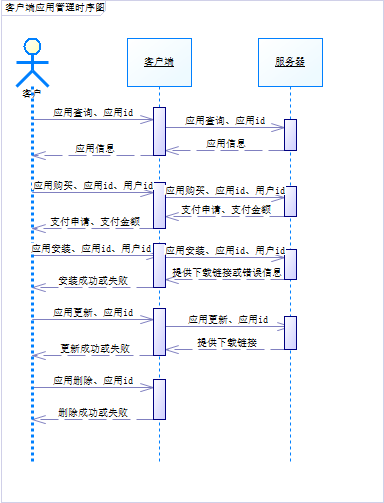
\includegraphics[width=14cm]{client_app_order.png}
	\caption{客户端进行应用管理的事件时序} \label{fig:client_app_order}
\end{figure}
见图\ref{fig:client_app_order}

\textbf{C. 对异常情况的回应}

\begin{longtable}{|c|p{6cm}|p{6cm}|}
\caption{客户端应用管理异常处理}\label{tab:client_app_management_exception}\\
\hline
\textbf{异常类型} & \textbf{异常描述} & \textbf{异常处理}\\
\hline
\endfirsthead

\hline
\textbf{异常类型} & \textbf{异常描述} & \textbf{异常处理}\\
\hline
\endhead
\hline 
\endfoot
\hline
\endlastfoot
服务器异常 & 
与服务器采用网络通信,限定时间内没有收到应答 &
储存错误状态,提示用户检查网络连接\\
应用id不合法 
& id对应的应用并不存在于本地(更新、删除),id对应的应用并不存在于应用商店(购买、安装、更新)
& 提示用户重新操作\\
本地磁盘空间不足
& 本地磁盘空间不足导致应用无法安装
& 提示用户释放本地磁盘空间\\
\end{longtable}

表\ref{tab:client_app_management_exception}概要性描述了几个可能出现的错误,以及相关的解决方案。
更加详细的方案见概要设计。

\textbf{D. 用于把系统输入转换到相应输出的任何方法}
只需要将服务器返回的结果返回给用户即可,不需要额外的数学算法或操作逻辑等等。
		
\textbf{E. 对输出数据的有效性检测}

此处只考虑客户端返回给客户的数据,返回给服务器的数据参见服务器端.用户管理系统。
输出数据为:操作的成功与否以及可能的错误信息,具体如下:
\begin{longtable}{|p{7cm}|p{7cm}|}
\caption{开发者端应用管理输出有效性检测}\label{tab:concrete_dev_sys_output_valid} \\
\hline
\textbf{输出内容} & \textbf{有效性检测} \\
\hline
\endfirsthead
\hline
\textbf{输出内容} & \textbf{有效性检测} \\
\hline
\endhead
\hline 
\endfoot
\hline
\endlastfoot

操作结果 & 布尔量,成功或失败 \\
查询结果 & 若干个元组,每个元组表示相关的应用的信息,可以为空\\
错误信息 & 操作成功则为空,操作失败则为一个字符串,建议开发者下一步的操作,长度暂定为128byte,具体参见对异常情况的回应部分\\
\end{longtable}


\subsubsection{输出}

需求编码为SRS\_User\_App\_P01\_O1

参见上一节E对输出数据的有效性检测。



\subsection{客户端.信息反馈}
本小节主要描述了普通用户进行信息反馈的需求,包括应用评分、评价等等。

需求编码为SRS\_User\_Info\_P01
\subsubsection{介绍}
逐条列出与本特性相关的功能需求。包括项目如何响应预期的错误输入,非法条件和无效输入。需求应该简明,完整,不含糊,可验证,必要的。 当需要的信息不确定的时候使用“待定”。

需求编码为SRS\_User\_Info\_P01\_F01

\subsubsection{输入}

针对客户对应用进行评价的需求,输入数据应当包括:应用id、评价、评分等等,数据来源均为客户,具体如下:

需求编码为SRS\_User\_Info\_P01\_I01

\begin{longtable}[]{@{}ll@{}}
\toprule
数据名称 & 数据要求\tabularnewline
\midrule
\endhead
应用id & 应用id为该客户本地已安装的应用之一\tabularnewline
评分 & 1-5之间的整型数字,可以为空\tabularnewline
评论 & 一个字符串,长度暂定为256字节,可以为空\tabularnewline
\bottomrule
\end{longtable}

\subsubsection{处理}
对输入进行处理,得到输出内容

需求编码为SRS\_User\_Info\_P01\_H01

\textbf{A. 输入数据的有效性检测}

\begin{longtable}[]{@{}ll@{}}
\caption{客户端信息反馈的输入数据的有效性检测}\label{tab:client_app_info}\\
\toprule
数据名称 & 数据要求\tabularnewline
\midrule
\endhead
具体需求 & 应用信息查询、评论回复、收入查询、收入提现、收入转账等命令之一\tabularnewline
应用id & 当且仅当具体需求是应用信息查询时不为空,应用id为该开发者开发的应用之一\tabularnewline
评论回复 & 当且仅当具体需求是评论回复时不为空,为一个字符串,长度暂定为256字节\tabularnewline
银行账号 & 当且仅当具体需求是收入提现或转账时不为空,为一个合法的银行账号\tabularnewline
\bottomrule
\end{longtable}

见表\ref{tab:client_app_info}

\textbf{B. 操作的确切次序,包括各事件的时序}

\begin{figure}[ht]
	\centering
	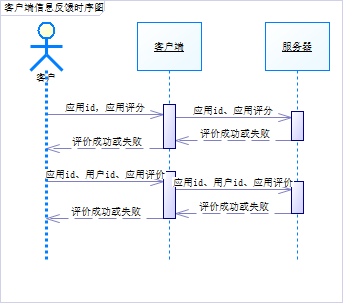
\includegraphics[width=14cm]{client_info_order.png}
	\caption{开发者获取信息反馈并处理的事件时序} \label{fig:client_info_order}
\end{figure}
见图\ref{fig:client_info_order}

\textbf{C. 对异常情况的回应}

\begin{longtable}{|c|p{6cm}|p{6cm}|}
\caption{开发者端信息反馈异常处理}\label{tab:client_info_exception}\\
\hline
\textbf{异常类型} & \textbf{异常描述} & \textbf{异常处理}\\
\hline
\endfirsthead

\hline
\textbf{异常类型} & \textbf{异常描述} & \textbf{异常处理}\\
\hline
\endhead
\hline 
\endfoot
\hline
\endlastfoot
服务器异常 & 
与服务器采用网络通信,限定时间内没有收到应答 &
储存错误状态,提示开发者检查网络连接\\
应用id不合法 
& id对应的应用并未在用户本地安装
& 提示开发者重新操作
\end{longtable}

表\ref{tab:client_info_exception}概要性描述了几个可能出现的错误,以及相关的解决方案。
更加详细的方案见概要设计。

\textbf{D. 用于把系统输入转换到相应输出的任何方法}
只需要将服务器返回的结果返回给用户即可,不需要额外的数学算法或操作逻辑等等。
		
\textbf{E. 对输出数据的有效性检测}

此处只考虑客户端返回给客户的数据,返回给服务器的数据参见服务器端.客户管理系统。具体如下:
\begin{longtable}{|p{7cm}|p{7cm}|}
\caption{客户端信息反馈输出有效性检测}\label{tab:concrete_dev_sys_output_valid} \\
\hline
\textbf{输出内容} & \textbf{有效性检测} \\
\hline
\endfirsthead
\hline
\textbf{输出内容} & \textbf{有效性检测} \\
\hline
\endhead
\hline 
\endfoot
\hline
\endlastfoot
操作结果 & 布尔量

\end{longtable}


\subsubsection{输出}
需求编码为SRS\_User\_Info\_P01\_O01

参见上一节E对输出数据的有效性检测。



{\color{red}

\subsection{客户端.应用个性化界面}

本小节主要描述了普通用户对应用进行配置并运行预览的界面。

需求编码为SRS\_User\_Dev\_P01
\subsubsection{介绍}

不同的用户对同一个应用可能有不同的需求,使用配置接口,设定不同的从参数,获得不同的
应用版本。

需求编码为SRS\_User\_Dev\_P01\_F01

\subsubsection{输入}

用户的输入主要是配置的参数,依据不同应用给出的接口而定。

同时应用的开发人员也需要明确指出不同的参数配置方式。并且与接口相接。

需求编码为SRS\_User\_Dev\_P01\_I01


\subsubsection{处理}
对输入进行处理,得到输出内容

需求编码为SRS\_User\_Dev\_P01\_H01

\textbf{A. 输入数据的有效性检测}

符合配置接口定义即可,无需其他有效性检测。

\textbf{B. 操作的确切次序,包括各事件的时序}

配置好的参数返回服务器,进行运行预览。

预览的结果返回本界面。

\textbf{C. 对异常情况的回应}

\begin{longtable}{|c|p{6cm}|p{6cm}|}
\caption{开发者端信息反馈异常处理}\label{tab:client_info_exception}\\
\hline
\textbf{异常类型} & \textbf{异常描述} & \textbf{异常处理}\\
\hline
\endfirsthead

\hline
\textbf{异常类型} & \textbf{异常描述} & \textbf{异常处理}\\
\hline
\endhead
\hline 
\endfoot
\hline
\endlastfoot
服务器异常 & 
与服务器采用网络通信,限定时间内没有收到应答 &
储存错误状态,提示开发者检查网络连接\\
应用id不合法 
& id对应的应用并未在用户本地安装
& 提示开发者重新操作
\end{longtable}

表\ref{tab:client_info_exception}概要性描述了几个可能出现的错误,以及相关的解决方案。
更加详细的方案见概要设计。

\textbf{D. 用于把系统输入转换到相应输出的任何方法}
只需要将服务器返回的结果返回给用户即可,不需要额外的数学算法或操作逻辑等等。
		
\textbf{E. 对输出数据的有效性检测}

此处只考虑客户端返回给客户的数据,返回给服务器的数据参见服务器端.客户管理系统。具体如下:
\begin{longtable}{|p{7cm}|p{7cm}|}
\caption{客户端信息反馈输出有效性检测}\label{tab:concrete_dev_sys_output_valid} \\
\hline
\textbf{输出内容} & \textbf{有效性检测} \\
\hline
\endfirsthead
\hline
\textbf{输出内容} & \textbf{有效性检测} \\
\hline
\endhead
\hline 
\endfoot
\hline
\endlastfoot
操作结果 & 布尔量

\end{longtable}


\subsubsection{输出}
需求编码为SRS\_User\_Dev\_P01\_O01

参见上一节E对输出数据的有效性检测。

}

\section{性能需求}

\subsection{开发者端性能}
需求编码为SRS\_NF\_P1\_E01

开发者端的性能主要依赖于服务器的性能,例如:上传、更新、删除应用的请求应当在1秒内得到相应,可以向服务器并行提交并执行多个请求。

\subsection{客户端性能}
需求编码为SRS\_NF\_P1\_E02

客户端的性能也主要依赖于服务器的性能,例如:对应用的查询、购买、安装等操作应当在1秒内得到相应。
但客户端还需要独自管理本地已安装的应用,这里要求客户端能够在1秒内列出本地所有通过应用商店安装的应用。

\subsection{服务器性能}
需求编码为SRS\_NF\_P1\_E03

本子章节应从整体上描述静态和动态的量化的对软件(或人与软件交互)的需求。

\begin{longtable}{|p{4cm}|p{10cm}|}
\caption{服务器性能}\label{tab:concrete_performance_server} \\
\hline
\textbf{性能需求} & \textbf{需求的具体内容}     \\
\hline
\endfirsthead
%\multicolumn{4}{c}{\tablename\ \thetable\ -- \textit{Continued from previous page}} \\
\hline
\textbf{性能需求} & \textbf{需求的具体内容}    \\
\hline
\endhead
\hline 
%\multicolumn{4}{r}{\textit{Continued on next page}} \\
\endfoot
\hline
\endlastfoot
支持的开发者数 & 100,000 \\
支持的用户数 & 1,000,000 \\
并发开发者数 & 1,000 \\
并发用户数 & 100,000 \\
应用大小限制 & 100G(更大的需要申请)\\
应用总数 & 100,000,000 \\
\end{longtable}

服务器的性能需求见表\ref{tab:concrete_performance_server}

\section{外部接口需求}
\subsection{用户接口}
需求编码为SRS\_UserInter\_01

\begin{longtable}{|p{4cm}|p{7cm}|p{7cm}|}
	\caption{开发者与应用商店系统的接口}\label{tab:developer_interface} \\
	\hline
	\textbf{开发者需求} & \textbf{输入} & \textbf{输出}\\
	\hline
	\endfirsthead
	\hline
	\textbf{开发者需求} & \textbf{输入} & \textbf{输出}\\
	\hline
	\endhead
	\hline 
	\endfoot
	\hline
	\endlastfoot
	登录 & 账号、密码 & 登录成功与否\\
	注册 & 账号、密码 & 注册成功与否\\
	应用上传 & 本地应用 & 上传成功与否\\
	应用更新 & 本地应用和待更新应用id & 更新成功与否\\
	应用删除 & 待删除应用id & 删除成功与否\\
	收入查询 & 无 & 收入\\
	评论回复 & 回复内容 & 回复成功与否\\
	\end{longtable}

\begin{longtable}{|p{4cm}|p{7cm}|p{7cm}|}
	\caption{普通用户与应用商店系统的接口}\label{tab:client_interface} \\
	\hline
	\textbf{用户需求} & \textbf{输入} & \textbf{输出}\\
	\hline
	\endfirsthead
	\hline
	\textbf{用户需求} & \textbf{输入} & \textbf{输出}\\
	\hline
	\endhead
	\hline 
	\endfoot
	\hline
	\endlastfoot
	登录 & 账号、密码 & 登录成功与否\\
	注册 & 账号、密码 & 注册成功与否\\
	应用查询 & 应用id & 相关的应用,以列表呈现\\
	应用购买 & 待购买应用id和银行账户 & 购买成功与否\\
	应用安装 & 待安装应用id & 安装成功与否\\
    应用删除 & 待删除应用id & 删除成功与否\\
	应用评分 & 待评价应用id和评分 & 评分成功与否\\
	应用评价 & 待评价应用id和评论 & 评论成功与否\\
	\end{longtable}
开发者和普通用户与该应用商店系统之间的接口分别参见表\ref{tab:developer_interface}和表\ref{tab:client_interface}。

输入、输出的时序关系参见之前的功能需求部分。

另外,应用商店系统的还包含help选项和一定的异常处理,提示开发者和普通用户如何正确操作。

\subsection{软件接口}

需求编码为SRS\_SoftInter\_01

该应用商店系统与外部有关联的软件只有操作系统和数据库。
\begin{longtable}{|p{4cm}|p{10cm}|}
\caption{操作系统与应用商店系统的接口}\label{tab:os_interface} \\
\hline
\textbf{接口目的} & \textbf{接口形式}\\
\hline
\endfirsthead
\hline
\textbf{接口目的} & \textbf{接口形式}\\
\hline
\endhead
\hline 
\endfoot
\hline
\endlastfoot
在本地安装应用 & bool install(package,loaction),package为软件包的文件描述符,location为安装目录\\
删除本地应用 & bool uninstall(uninstallProgram),uninstallProgram为卸载程序的文件描述符\\
\end{longtable}

\begin{longtable}{|p{4cm}|p{10cm}|}
	\caption{数据库与应用商店系统的接口}\label{tab:db_interface} \\
	\hline
	\textbf{接口目的} & \textbf{接口形式}\\
	\hline
	\endfirsthead
	\hline
	\textbf{接口目的} & \textbf{接口形式}\\
	\hline
	\endhead
	\hline 
	\endfoot
	\hline
	\endlastfoot
	查询应用信息 & app searchApp(id),id为应用id,app为一个结构体,包含了有关该应用的信息\\
	查询用户信息 & client searchClient(account),account为用户账号,client为一个结构体,包含了有关该用户的信息\\
	查询开发者信息 & developer searchDeveloper(account),account为开发者账号,developer为一个结构体,包含了有关该开发者的信息\\
	修改应用信息 & bool updateApp(app),app为一个结构体,也可用此接口新增应用\\
	修改用户信息 & bool updateClient(client),client为一个结构体,也可用此接口新增用户\\
	修改开发者信息 & bool updateDeveloper(developer),developer为一个结构体,也可用此接口新增开发者\\
	\end{longtable}
该应用商店系统和操作系统及数据库的接口分别参见表\ref{tab:os_interface}和表\ref{tab:db_interface}。

\subsection{硬件接口}

需求编码为SRS\_HardInter\_01

该应用商店系统不需要使用外部的硬件设备如打印机等等,故无需考虑硬件接口。

\subsection{通讯接口}

需求编码为SRS\_CommInter\_01

服务器端、客户端和开发者端之间的通信均采用TCP/IP协议。
\chapter{总体设计约束}
本节描述了对开发人员开发本系统的一些限制。
 
\section{标准符合性}
开发过程中的以下内容应遵从如下标准:\\
\begin{longtable}{|p{4cm}|p{10cm}|}
\caption{采用的标准和规范}\label{tab:standards_constraints} \\
\hline
内容 & 标准或规范\\
\hline
字符集 & utf-8\\
网络协议 & RFC\\
\hline
\end{longtable}





\section{硬件约束}
该应用商店可在Windows、Macintosh、Linux、Android、iOS、web等多种平台上运行,在不同平台上的约束要求如下:\\

\begin{longtable}{|p{4cm}|p{10cm}|}
\caption{在不同平台运行的需求}\label{tab:hardware_constraints} \\
\hline
\textbf{平台} & \textbf{需求}     \\
\hline
\endfirsthead
\hline
\textbf{平台} & \textbf{需求}    \\
\hline
\endhead
\hline 
\endfoot
\hline
\endlastfoot
Windows & 内存占用不超过100MB,存储空间占用不超过100MB \\
Macintosh & 内存占用不超过100MB,存储空间占用不超过100MB \\
Linux & 内存占用不超过100MB,存储空间占用不超过100MB \\
Android & 内存占用不超过200MB,存储空间占用不超过100MB\\
iOS & 内存占用不超过100MB,存储空间占用不超过200MB\\
web & 内存占用不超过100MB \\
\end{longtable}

\section{技术限制}
本节描述了开发人员在开发该应用商店系统时使用的技术限制。\\
\begin{longtable}{|p{4cm}|p{10cm}|}
\caption{技术限制}\label{tab:technical_constraints} \\
\hline
技术 & 限制\\
\hline
数据库 & Oracle数据库\\
通讯协议 & 客户端、服务器、开发者端之间的通信均采用TCP协议\\
编程规范 & 采用Google代码规范,详见https://zh-google-styleguide.readthedocs.io/en/latest/contents/\\
\hline
\end{longtable}

\chapter{软件质量特性}
本节描述了该应用商店系统应当具备的软件质量特性。
\section{功能性}
\subsection{适合性和和准确性}
本系统针对开发者和普通用户的需求进行开发,分为开发者端、客户端和服务器端,应当完全可以满足开发者开发、管理应用和普通用户使用、管理应用的各种需求。
\subsection{保密安全性}
开发者和普通用户均需要登录账户才可以正常地访问数据并进行各种操作(普通用户查询应用和管理本地已安装应用除外),禁止未授权的用户访问和操作。

\section{可靠性}
该应用商店系统能够处理一定的异常,详见3.1功能需求部分的描述。对于未知类型的异常,软件应当能够保存发生异常的状态,使得能够从异常中恢复,并将该未知异常上传给服务器,以便开发人员修复。

\section{易用性}
无论是开发者端、客户端还是服务器端,该系统的各种操作都应当有明确的提示信息和操作说明。另外,对于开发者端和客户端而言,交互界面还应当美观,操作逻辑清晰简洁,便于开发者和普通用户使用。

\section{效率性}
该应用商店系统能够在给定的资源下处理一定的事务,详见3.2性能需求部分的描述。

\section{可维护性}
\subsection{易分析性和易改变性}
该应用商店系统的各个模块应当合理划分,使得当出现问题时能够快速定位问题所在,也使得后续可能的需求变更能够更容易地实现。
\subsection{稳定性}
开发过程应采用增量开发,防止意外修改导致软件失效。
\subsection{易测试性}
该应用商店系统的各个模块的输出应当足够明确和完备,以便确认软件的功能是否正确实现。

\section{可移植性}
\subsection{适应性}
该应用商店系统能够适应不同的平台,包括Windows、Macintosh、Linux、Android、iOS、web等等。
\subsection{易安装性}
该应用商店系统应当提供类似能够“一键安装”的安装包,便于开发者和普通用户使用。



\chapter{其他需求}

使用适当的章节,详细说明任何其他客户需求,包括数据库,编码需求,错误处理,测试需求等。

需求编码为SRS\_NF\_P02

\section{数据库}

需求编码为SRS\_NF\_P02\_E01
{\color{red}

\subsection{检索速度v.s.稳定性}
本应用并不强调检索的速度,因为应用的数量并不会过多,所以更多地从稳定性考虑。


    从稳定性考虑,本系统的数据系统采用Oracle 12数据库系统;使用centOS作为
    操作系统。

\subsection{数据一致性考虑}
本系统同时也不强调一致性,应用的开发、应用的下载并不是冲突的操作。

用户下载的应用仅仅是系统中的最新版本即可。

}


\section{本地化}
内置语言转化:汉语、英语、法语、俄语、日语、德语,阿拉伯语、西班牙语;

默认为:系统语言

需求编码为SRS\_NF\_P02\_L01

\section{扩展性}
应该允许普通的开发人员参与本系统的完善与改进

需求编码为SRS\_NF\_P02\_S01

\section{开源性}
开发人员可以选择是否开源,并选择合适的开源许可证,本系统应该同时提供各种开源许可的简介与详细内容。

需求编码为SRS\_NF\_P02\_K01

\section{开发者与用户关系}
不应严格区分开发者与用户,即一个邮箱帐号可同时为用户与开发者。

需求编码为SRS\_NF\_P02\_R01

\chapter{依赖关系}
每条需求的内部和外部依赖关系列表如下:

\begin{longtable}{|p{6cm}|p{6cm}|p{6cm}}
\caption{需求的内外部依赖关系}\label{tab:concrete_dev_sys_output_valid} \\
\hline
\textbf{需求} & \textbf{内部依赖} & \textbf{外部依赖}\\
\hline
\endfirsthead
\hline
\textbf{需求} & \textbf{内部依赖} & \textbf{外部依赖}\\
\hline
\endhead
\hline 
\endfoot
\hline
\endlastfoot
开发者端.应用管理 & 服务器端.开发者管理系统和服务器端.应用管理系统 & 无\\
开发者端.信息反馈 & 服务器端.开发者管理系统和服务器端.应用管理系统 & 无\\
客户端.应用管理 & 服务器端.客户管理系统和服务器端.应用管理系统 & 无\\
客户端.信息反馈 &
服务器端.客户管理系统和服务器端.应用管理系统 & 无\\
服务器端.开发者管理系统 & 服务器端.应用管理系统 & 数据库\\
服务器端.用户管理系统 & 服务器端.应用管理系统 & 数据库\\
服务器端.应用管理系统 & 服务器端.开发者管理系统和服务器端.用户管理系统 & 数据库\\ 
服务器端.第三方管理系统 & 无 & 数据库\\ 

\end{longtable}
\chapter{需求分级}

\begin{longtable}{|p{6cm}|p{6cm}|c|}
\caption{需求分级表} \label{tab:classification}\\
\hline
\textbf{需求ID} & \textbf{需求名称} & \textbf{需求分级}\\
\hline
\endfirsthead

\hline
\textbf{需求ID} & \textbf{需求名称} & \textbf{需求分级}\\
\hline
\endhead
\hline 
\endfoot
\hline
\endlastfoot
SRS\_Dev\_App\_P01 & 开发者端的应用管理 & A \\
\hline
SRS\_Dev\_Info\_P01 & 开发者端的信息反馈 & B \\
\hline
{\color{red}SRS\_Dev\_Dev\_P01} & {\color{red}开发者端应用开发界面} & {\color{red}A} \\
\hline
SRS\_Server\_Dev\_P01 & 服务器端的开发者管理 & A \\
\hline
SRS\_Server\_User\_P01 & 服务器端的用户管理 & A \\
\hline
SRS\_Server\_Other\_P01 & 服务器端的第三方管理 & B \\
\hline
{\color{red}SRS\_Server\_DevSys\_P01} & {\color{red}服务器端应用开发管理系统} & {\color{red}A} \\
\hline
SRS\_User\_App\_P01 & 用户端的应用管理 & A \\
\hline
SRS\_User\_Info\_P01 & 用户端的信息反馈 & B \\
\hline
{\color{red}SRS\_User\_Dev\_P01} & {\color{red}客户端应用个性化系统} & {\color{red}A} \\
\hline
SRS\_NF\_P1\_E01 & 开发者端性能 & B \\
\hline
SRS\_NF\_P1\_E02 & 客户端性能 & B \\
\hline
SRS\_NF\_P1\_E03 & 服务器性能 & B \\
\hline
SRS\_UserInter\_01 & 用户接口 & A \\
\hline
SRS\_SoftInter\_01 & 软件接口 & A \\
\hline
SRS\_HardInter\_01 & 硬件接口 & A \\
\hline
SRS\_CommInter\_01 & 通讯接口 & A \\
\hline
SRS\_NF\_P02\_E01 & 数据库 & C \\
\hline
SRS\_NF\_P02\_L01 & 本地化 & C \\
\hline
SRS\_NF\_P02\_S01 & 扩展性 & C \\
\hline
SRS\_NF\_P02\_K01 & 开源性 & C \\
\hline
SRS\_NF\_P02\_R01 & 开发者与用户关系 & C \\
\end{longtable}

重要性分类如下:
\begin{itemize}
\item A:(必须的)		绝对基本的特性;如果不包含,产品就会被取消。
\item B:(重要的)		不是基本的特性,但这些特性会影响产品的生存能力。
\item C:(最好有的)		期望的特性;但省略一个或多个这样的特性不会影响产品的生存能力
\end{itemize}

\chapter{待确定问题}
\begin{table}[htbp]
\centering
\caption{待确定问题表} \label{tab:tbd_problems}
\begin{tabular}{|c|c|c|c|c|c|c|}
    \hline %状态(Open/Close) 
    需求ID & 问题描述 & 影响(H/M/L) & 风险 & 责任人 & 解决日期 & 状态 \\
    \hline
    SRS\_Dev\_App\_P01 & 应用格式转换 & H & 高 & 李楠 &  & Open\\
    \hline
    SRS\_Server\_Other\_P01 & 可拓展性 & M & 低 & 董恒 & 2019/5/2 & Close\\
    \hline
\end{tabular}
\end{table}
%\chapter{Latex使用例子}

\section{图}
\subsection{示例}
\begin{figure}[ht]
\centering

\includegraphics[width=10cm]{ustc_logo_fig}
\caption{测试图片} \label{fig:figure1}
\end{figure}

\subsection{带图注的图}
\begin{figure}[ht]
\centering

\includegraphics[width=10cm]{ustc_logo_fig}
\caption{带图注的图片}\label{fig:noted-figure}
\note{the solid lines represent the time histogram of the spontaneous activities of an old monkey cell(gray) and a young monkey cell (black). The bin-width is 1}
\end{figure}

\section{表格}

\subsection{A Simple Table}
\begin{table}[htbp]
\centering
\caption{这里是表的标题} \label{tab:simpletable}
\begin{tabular}{|c|c|}
    \hline
    a & b \\
    \hline
    c & d \\
    \hline
\end{tabular}
\note{这里是表的注释}
\end{table}

\subsection{长表格}
\begin{longtable}{ccc}
% 首页表头
\caption[长表格演示]{长表格演示} \label{tab:longtable} \\
\toprule[1.5pt]
名称  & 说明 & 备注\\
\midrule[1pt]
\endfirsthead
% 续页表头
\caption[]{长表格演示(续)} \\
\toprule[1.5pt]
名称  & 说明 & 备注 \\
\midrule[1pt]
\endhead
% 首页表尾
\hline
\multicolumn{3}{r}{\small 续下页}
\endfoot
% 续页表尾
\bottomrule[1.5pt]
\endlastfoot

AAAAAAAAAAAA   &   BBBBBBBBBBB   &   CCCCCCCCCCCCCC   \\
AAAAAAAAAAAA   &   BBBBBBBBBBB   &   CCCCCCCCCCCCCC   \\
AAAAAAAAAAAA   &   BBBBBBBBBBB   &   CCCCCCCCCCCCCC   \\
AAAAAAAAAAAA   &   BBBBBBBBBBB   &   CCCCCCCCCCCCCC   \\
AAAAAAAAAAAA   &   BBBBBBBBBBB   &   CCCCCCCCCCCCCC   \\
AAAAAAAAAAAA   &   BBBBBBBBBBB   &   CCCCCCCCCCCCCC   \\
AAAAAAAAAAAA   &   BBBBBBBBBBB   &   CCCCCCCCCCCCCC   \\
AAAAAAAAAAAA   &   BBBBBBBBBBB   &   CCCCCCCCCCCCCC   \\
AAAAAAAAAAAA   &   BBBBBBBBBBB   &   CCCCCCCCCCCCCC   \\
AAAAAAAAAAAA   &   BBBBBBBBBBB   &   CCCCCCCCCCCCCC   \\
AAAAAAAAAAAA   &   BBBBBBBBBBB   &   CCCCCCCCCCCCCC   \\
AAAAAAAAAAAA   &   BBBBBBBBBBB   &   CCCCCCCCCCCCCC   \\
AAAAAAAAAAAA   &   BBBBBBBBBBB   &   CCCCCCCCCCCCCC   \\
AAAAAAAAAAAA   &   BBBBBBBBBBB   &   CCCCCCCCCCCCCC   \\
AAAAAAAAAAAA   &   BBBBBBBBBBB   &   CCCCCCCCCCCCCC   \\
AAAAAAAAAAAA   &   BBBBBBBBBBB   &   CCCCCCCCCCCCCC   \\
AAAAAAAAAAAA   &   BBBBBBBBBBB   &   CCCCCCCCCCCCCC   \\
AAAAAAAAAAAA   &   BBBBBBBBBBB   &   CCCCCCCCCCCCCC   \\
AAAAAAAAAAAA   &   BBBBBBBBBBB   &   CCCCCCCCCCCCCC   \\
AAAAAAAAAAAA   &   BBBBBBBBBBB   &   CCCCCCCCCCCCCC   \\
AAAAAAAAAAAA   &   BBBBBBBBBBB   &   CCCCCCCCCCCCCC   \\
AAAAAAAAAAAA   &   BBBBBBBBBBB   &   CCCCCCCCCCCCCC   \\
AAAAAAAAAAAA   &   BBBBBBBBBBB   &   CCCCCCCCCCCCCC   \\
AAAAAAAAAAAA   &   BBBBBBBBBBB   &   CCCCCCCCCCCCCC   \\
AAAAAAAAAAAA   &   BBBBBBBBBBB   &   CCCCCCCCCCCCCC   \\
AAAAAAAAAAAA   &   BBBBBBBBBBB   &   CCCCCCCCCCCCCC   \\
AAAAAAAAAAAA   &   BBBBBBBBBBB   &   CCCCCCCCCCCCCC   \\
AAAAAAAAAAAA   &   BBBBBBBBBBB   &   CCCCCCCCCCCCCC   \\
AAAAAAAAAAAA   &   BBBBBBBBBBB   &   CCCCCCCCCCCCCC   \\
AAAAAAAAAAAA   &   BBBBBBBBBBB   &   CCCCCCCCCCCCCC   \\
AAAAAAAAAAAA   &   BBBBBBBBBBB   &   CCCCCCCCCCCCCC   \\
AAAAAAAAAAAA   &   BBBBBBBBBBB   &   CCCCCCCCCCCCCC   \\
AAAAAAAAAAAA   &   BBBBBBBBBBB   &   CCCCCCCCCCCCCC   \\
AAAAAAAAAAAA   &   BBBBBBBBBBB   &   CCCCCCCCCCCCCC   \\
AAAAAAAAAAAA   &   BBBBBBBBBBB   &   CCCCCCCCCCCCCC   \\
AAAAAAAAAAAA   &   BBBBBBBBBBB   &   CCCCCCCCCCCCCC   \\
\end{longtable}


\section{算法环境}
模板中使用 \texttt{algorithm2e} 宏包实现算法环境。关于该宏包的具体用法,
请阅读宏包的官方文档。

\begin{algorithm}[htbp]
\SetAlgoLined
\KwData{this text}
\KwResult{how to write algorithm with \LaTeX2e }

initialization\;
\While{not at end of this document}{
    read current\;
    \eIf{understand}{
        go to next section\;
        current section becomes this one\;
    }{
        go back to the beginning of current section\;
    }
}
\caption{算法示例1}
\label{algo:algorithm1}
\end{algorithm}

\IncMargin{1em}
\begin{algorithm}
\SetKwData{Left}{left}\SetKwData{This}{this}\SetKwData{Up}{up}
\SetKwFunction{Union}{Union}\SetKwFunction{FindCompress}{FindCompress}
\SetKwInOut{Input}{input}\SetKwInOut{Output}{output}

\Input{A bitmap $Im$ of size $w\times l$}
\Output{A partition of the bitmap}
\BlankLine
\emph{special treatment of the first line}\;
\For{$i\leftarrow 2$ \KwTo $l$}{
    \emph{special treatment of the first element of line $i$}\;
    \For{$j\leftarrow 2$ \KwTo $w$}{\label{forins}
        \Left$\leftarrow$ \FindCompress{$Im[i,j-1]$}\;
        \Up$\leftarrow$ \FindCompress{$Im[i-1,]$}\;
        \This$\leftarrow$ \FindCompress{$Im[i,j]$}\;
        \If(\tcp*[h]{O(\Left,\This)==1}){\Left compatible with \This}{\label{lt}
            \lIf{\Left $<$ \This}{\Union{\Left,\This}}
            \lElse{\Union{\This,\Left}}
        }
        \If(\tcp*[f]{O(\Up,\This)==1}){\Up compatible with \This}{\label{ut}
        \lIf{\Up $<$ \This}{\Union{\Up,\This}}
        \tcp{\This is put under \Up to keep tree as flat as possible}\label{cmt}
        \lElse{\Union{\This,\Up}}\tcp*[h]{\This linked to \Up}\label{lelse}
        }
    }
    \lForEach{element $e$ of the line $i$}{\FindCompress{p}}
}
\caption{算法示例2}\label{algo_disjdecomp}
\label{alog:algorithm2}
\end{algorithm}\DecMargin{1em}


\section{代码环境}
模板中使用 \texttt{listings} 宏包实现代码环境。详细用法见宏包的官方说明文档。

以下是代码示例,可以在文中任意位置引用\autoref{first-code} 。
\begin{lstlisting}[language=C, caption=示例代码, label={code:first-code}]
#include <stdio.h>

int main( )
{
    printf("hello, world\n");
    return 0;
}
\end{lstlisting}




\section{引用文献标注}

\subsection{著者-出版年制标注法}

\noindent
\verb|\citestyle{ustcauthoryear}|
\citestyle{ustcauthoryear}

\noindent
\begin{tabular}{l@{\quad$\Rightarrow$\quad}l}
  \verb|\cite{knuth86a}| & \cite{knuth86a}\\
  \verb|\citet{knuth86a}| & \citet{knuth86a}\\
  \verb|\citet[chap.~2]{knuth86a}| & \citet[chap.~2]{knuth86a}\\[0.5ex]
  \verb|\citep{knuth86a}| & \citep{knuth86a}\\
  \verb|\citep[chap.~2]{knuth86a}| & \citep[chap.~2]{knuth86a}\\
  \verb|\citep[see][]{knuth86a}| & \citep[see][]{knuth86a}\\
  \verb|\citep[see][chap.~2]{knuth86a}| & \citep[see][chap.~2]{knuth86a}\\[0.5ex]
  \verb|\citet*{knuth86a}| & \citet*{knuth86a}\\
  \verb|\citep*{knuth86a}| & \citep*{knuth86a}\\
\end{tabular}

\noindent
\begin{tabular}{l@{\quad$\Rightarrow$\quad}l}
  \verb|\citet{knuth86a,tlc2}| & \citet{knuth86a,tlc2}\\
  \verb|\citep{knuth86a,tlc2}| & \citep{knuth86a,tlc2}\\
  \verb|\cite{knuth86a,knuth84}| & \cite{knuth86a,knuth84}\\
  \verb|\citet{knuth86a,knuth84}| & \citet{knuth86a,knuth84}\\
  \verb|\citep{knuth86a,knuth84}| & \citep{knuth86a,knuth84}\\
\end{tabular}

\subsection{顺序编码制标注法}

\noindent
\verb|\citestyle{ustcnumerical}|
\citestyle{ustcnumerical}

\noindent
\begin{tabular}{l@{\quad$\Rightarrow$\quad}l}
  \verb|\cite{knuth86a}| & \cite{knuth86a}\\
  \verb|\citet{knuth86a}| & \citet{knuth86a}\\
  \verb|\citet[chap.~2]{knuth86a}| & \citet[chap.~2]{knuth86a}\\[0.5ex]
  \verb|\citep{knuth86a}| & \citep{knuth86a}\\
  \verb|\citep[chap.~2]{knuth86a}| & \citep[chap.~2]{knuth86a}\\
  \verb|\citep[see][]{knuth86a}| & \citep[see][]{knuth86a}\\
  \verb|\citep[see][chap.~2]{knuth86a}| & \citep[see][chap.~2]{knuth86a}\\[0.5ex]
  \verb|\citet*{knuth86a}| & \citet*{knuth86a}\\
  \verb|\citep*{knuth86a}| & \citep*{knuth86a}\\
\end{tabular}

\noindent
\begin{tabular}{l@{\quad$\Rightarrow$\quad}l}
  \verb|\citet{knuth86a,tlc2}| & \citet{knuth86a,tlc2}\\
  \verb|\citep{knuth86a,tlc2}| & \citep{knuth86a,tlc2}\\
  \verb|\cite{knuth86a,knuth84}| & \cite{knuth86a,knuth84}\\
  \verb|\citet{knuth86a,knuth84}| & \citet{knuth86a,knuth84}\\
  \verb|\citep{knuth86a,knuth84}| & \citep{knuth86a,knuth84}\\
  \verb|\cite{knuth86a,knuth84,tlc2}| & \cite{knuth86a,knuth84,tlc2}\\
\end{tabular}

\subsection{其他形式的标注}

\noindent
\begin{tabular}{l@{\quad$\Rightarrow$\quad}l}
  \verb|\citealt{tlc2}| & \citealt{tlc2}\\
  \verb|\citealt*{tlc2}| & \citealt*{tlc2}\\
  \verb|\citealp{tlc2}| & \citealp{tlc2}\\
  \verb|\citealp*{tlc2}| & \citealp*{tlc2}\\
  \verb|\citealp{tlc2,knuth86a}| & \citealp{tlc2,knuth86a}\\
  \verb|\citealp[pg.~32]{tlc2}| & \citealp[pg.~32]{tlc2}\\
  \verb|\citenum{tlc2}| & \citenum{tlc2}\\
  \verb|\citetext{priv.\ comm.}| & \citetext{priv.\ comm.}\\
\end{tabular}

\noindent
\begin{tabular}{l@{\quad$\Rightarrow$\quad}l}
  \verb|\citeauthor{tlc2}| & \citeauthor{tlc2}\\
  \verb|\citeauthor*{tlc2}| & \citeauthor*{tlc2}\\
  \verb|\citeyear{tlc2}| & \citeyear{tlc2}\\
  \verb|\citeyearpar{tlc2}| & \citeyearpar{tlc2}\\
\end{tabular}

\bibliography{bib/tex}

\appendix
\chapter{可行性分析结果}
本节主要描述了开发这样一个应用商店系统的可行性分析结果。

\section{技术可行性}
由于现实中已经存在了一些相对较为成熟的应用商店系统,比如Microsoft Store,App Store,Google Play Store等等,因此从技术上来讲,必定是可以实现的。

下面粗略考虑各个需求的技术可行性。

服务器端可以用C++、Java、Python、PHP等各种编程语言编写,数据库可以使用Oracle数据库。

客户端和开发者端本质上是一样的,如果采用C/S架构,则可采用C++、Java、Python等语言编写,如果采用B/S架构,则可采用JavaScript,JSP等语言编写。不涉及数据库。

\section{非技术可行性}
\subsection{经济可行性}
初步的开发并不需要太多的人力和物力,在经济上是完全可行的。
\subsection{法律可行性}
该应用商店系统不会收集普通用户和开发者的个人信息用作商业用途,并保护开发者所开发的应用的版权,不会让其在未经开发者允许的情况下随意传播,因此是符合法律规定的。

\chapter{需求建模 }
\section{数据流图}
\subsection{顶层数据流图}
%top_level_DFD.png
\begin{figure}[ht]
	\centering
	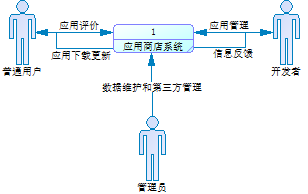
\includegraphics[width=7cm]{top_level_DFD.png}
	\caption{顶层数据流图} \label{fig:top_level_DFD}
\end{figure}
见图\ref{fig:top_level_DFD}

\subsection{0层数据流图}
\begin{figure}[ht]
	\centering
	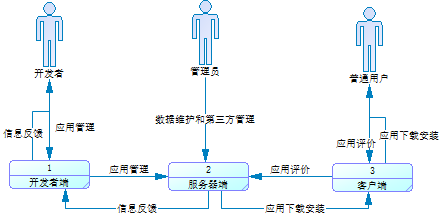
\includegraphics[width=10cm]{0_level_DFD.png}
	\caption{0层数据流图} \label{fig:0_level_DFD}
\end{figure}
见图\ref{fig:0_level_DFD}

\subsection{1层数据流图}
\begin{figure}[ht]
	\centering
	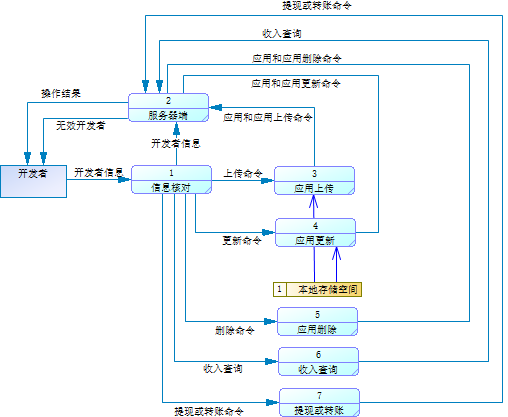
\includegraphics[width=12cm]{1_level_DFD_developer.png}
	\caption{1层数据流图-开发者端} \label{fig:1_level_DFD_dveloper}
\end{figure}
开发者端的1层数据流图见图\ref{fig:1_level_DFD_dveloper}

\begin{figure}[ht]
	\centering
	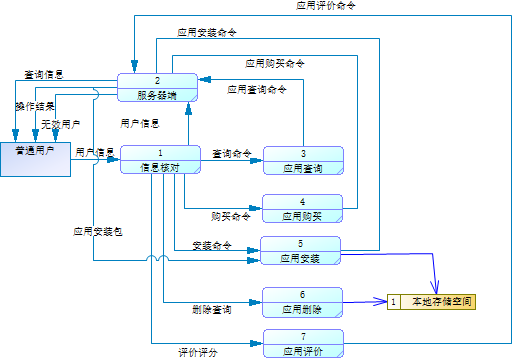
\includegraphics[width=12cm]{1_level_DFD_client.png}
	\caption{1层数据流图-客户端} \label{fig:1_level_DFD_client}
\end{figure}

客户端的1层数据流图见图\ref{fig:1_level_DFD_client}


%1_level_DFD_server.png
\begin{figure}[ht]
	\centering
	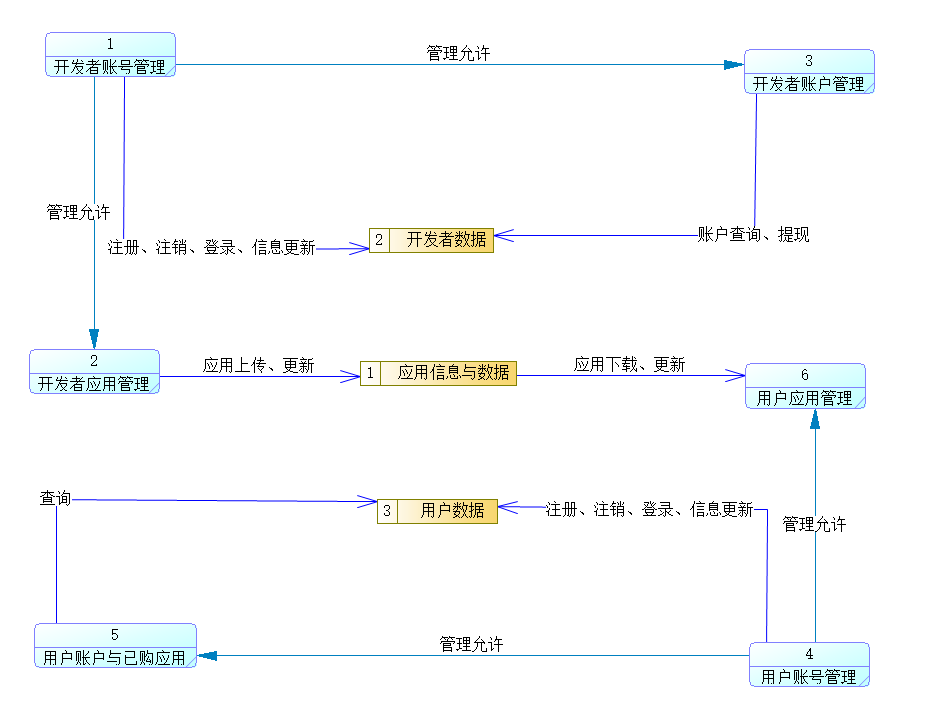
\includegraphics[width=12cm]{1_level_DFD_server.png}
	\caption{1层数据流图-服务器端} \label{fig:1_level_DFD_server}
\end{figure}

服务器的1层数据流图见图\ref{fig:1_level_DFD_server}

\section{数据字典}
\subsection{数据流说明}
\subsubsection{应用上载}

描述:开发者上传开发的应用

来源:开发者端

去处:服务器端(应用管理系统)

组成:应用ID+应用名+应用版本+应用描述+应用代码+开发者ID

\subsubsection{应用下载}

描述:用户下载应用

来源:服务器端(应用管理系统)

去处:客户端

组成:应用ID+应用名+应用版本+应用描述+可执行文件

\subsection{数据存储说明}
\subsubsection{应用}

流入数据流:添加、更新应用

流出数据流:检索、下载应用

组成:应用ID+应用名+应用版本+应用描述+应用代码+开发者ID+可执行文件

描述:应用的全部数据和信息

组织:按照特定类别排序

\subsubsection{用户信息}

流入数据流:用户注册、更新信息

流出数据流:用户登录

组成:用户ID+密码+基本信息+账户金额+已购买的应用

描述:用户的全部数据和信息

组织:按照用户ID排序

\subsubsection{开发者信息}

流入数据流:开发者注册、更新信息

流出数据流:开发者登录

组成:开发者ID+密码+基本信息+账户金额+开发的应用

描述:开发者的全部数据和信息

组织:按照开发者ID排序

\subsection{加工说明}
\subsubsection{应用检查}

\begin{lstlisting}[language=C, caption=示例代码, label={code:app_check}]
if(!secure_check(app)){
	return error.msg("not safe\n");
}
if(block_dev.has(app.info.dev)){
	return error.msg("blocked developer\n");
}
if(!running_test(app)){
	return error.msg("running error\n");
}
for(auto exist_app:app_list){
	if(similar_app(app,exist_app)>threshold){
		return error.msg("already exist app\n");
	}
}
app_list.push(app);

\end{lstlisting}

代码见\autoref{code:app_check} 




\end{document}
